
\section{Scalability Campaign}\label{results:scale}

Given the base parameter values described in Tables \ref{tbl:front_ref_params}
and \ref{tbl:back_ref_params}, exchanges were generated by scaling the number of
reactors in the system. The smallest system modeled included five reactors. The
largest exchanges included five-hundred reactors, a value chosen because there
are approximately five-hundred reactors currently operating (437) or under
construction (71) in the world \cite{nrxtrs}. Therefore, the largest exchanges
modeled represent a time step in a simulation in which the world-wide fleet of
reactors are all supplying or consuming a batch of fuel.

Front and back-end exchanges are explored similarly in the scalability
campaign. First, for all 18 combinations of fundamental parameters and each
solver, a set of reference cases are established, where the only varying
parameter is the number of reactors. Next, specific instance parameters are
chosen to vary in order to determine first-order effects as the exchange system
size scales. Finally, the effect of convergence criteria for the CBC solver is
investigated.

Individual figures for each experiment are provided for each fuel cycle modeled
($f_\text{fc}$) and each solver. Each figure summarizes the results for all
combinations of $f_\text{rx}$ and $f_\text{loc}$. The layout for each six-pane
figure is shown below.

\begin{figure}[h!]
  \begin{center}
    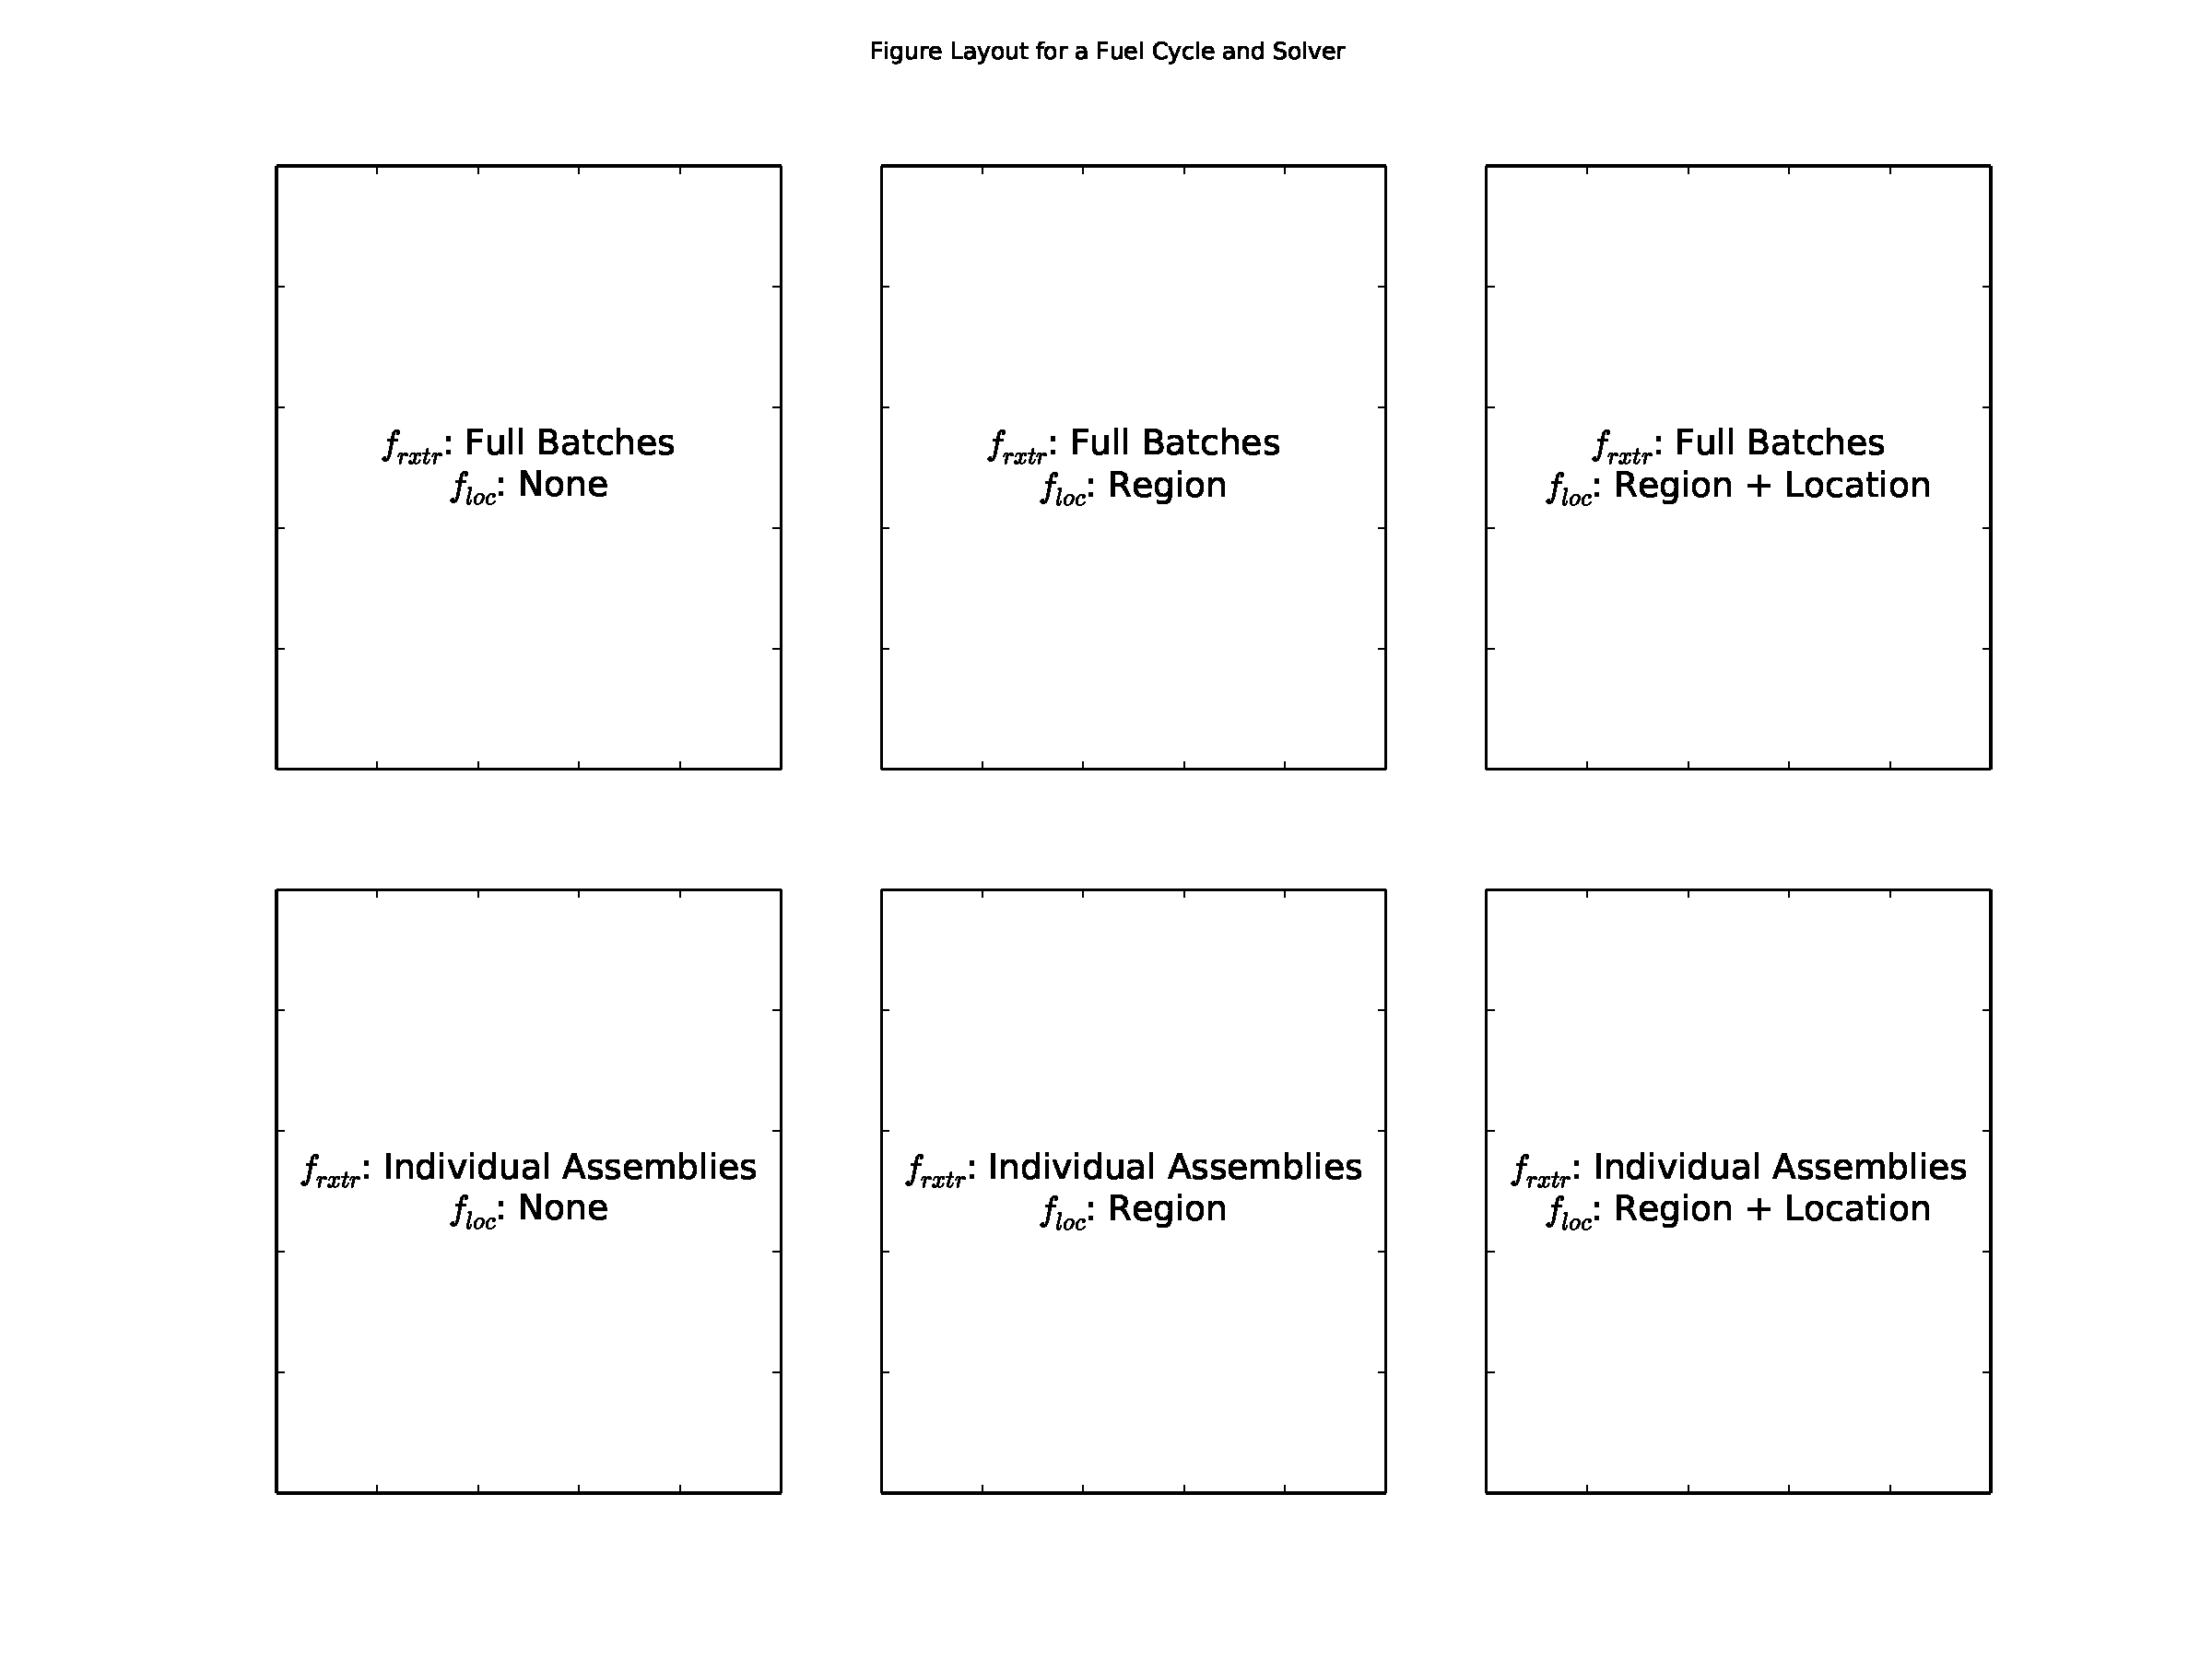
\includegraphics[width=.7\textwidth]{figure_layout.pdf}
    \caption[]{
      \label{fig:figure_layout}
      The general figure layout displaying results for different fundamental
      parameter values.}
  \end{center}
\end{figure}

\subsection{Front-End Exchanges}

\subsubsection{Reference Case}

Reference cases were generated for front-end exchanges by scaling the number of
reactors in each exchange. A step size of 5 reactors was used for the range of
$[5, 100]$ and a step size of 25 was used from $(100, 500]$. In mathematical
  programming, the number of variables and number of constraints in a problem
  are measures of problem scaling. In the NFCTP, constraints are provided by
  trading entities, and the number of variables is equal to the number of arcs
  in a given exchange graph. Accordingly, understanding how each quantiy scales
  with the number of reactors is of chief import.

Figure \ref{fig:base_front_n_rxtr_n_arcs_fc1_solvergreedy} shows how the number
of arcs scale with problem size for the MOX fuel cycle, and Figure
\ref{fig:base_front_n_rxtr_n_constrs_fc1_solvergreedy} shows the same results
for the number of constraints. The number of constraints scales linearly, for it
is a purely function of the number of entities in an exchange. However, the
number of arcs scales by $\mathcal{O}(n^2)$. During exchange generation, the
number of suppliers is a function of the number of reactors. Further, each
reactor and each supplier have an arc connecting them if the reactor can consume
the supplier's commodity. Therefore, adding a single reactor to the system
results in additional arcs for every reactor previously existing in the system,
resulting in an $\mathcal{O}(n^2)$ relationship. Both relationships hold true
regardless of the fuel cycle being modeled, and, as can be seen, are also
independent of other fundamental parameters. The arc population magnitude,
however, is a function of $f_\text{rxtr}$. As $f_\text{rxtr}$ increases, $n_a$
individual assemblies are requested rather than a single batch.

\begin{figure}[h!]
  \begin{center}
    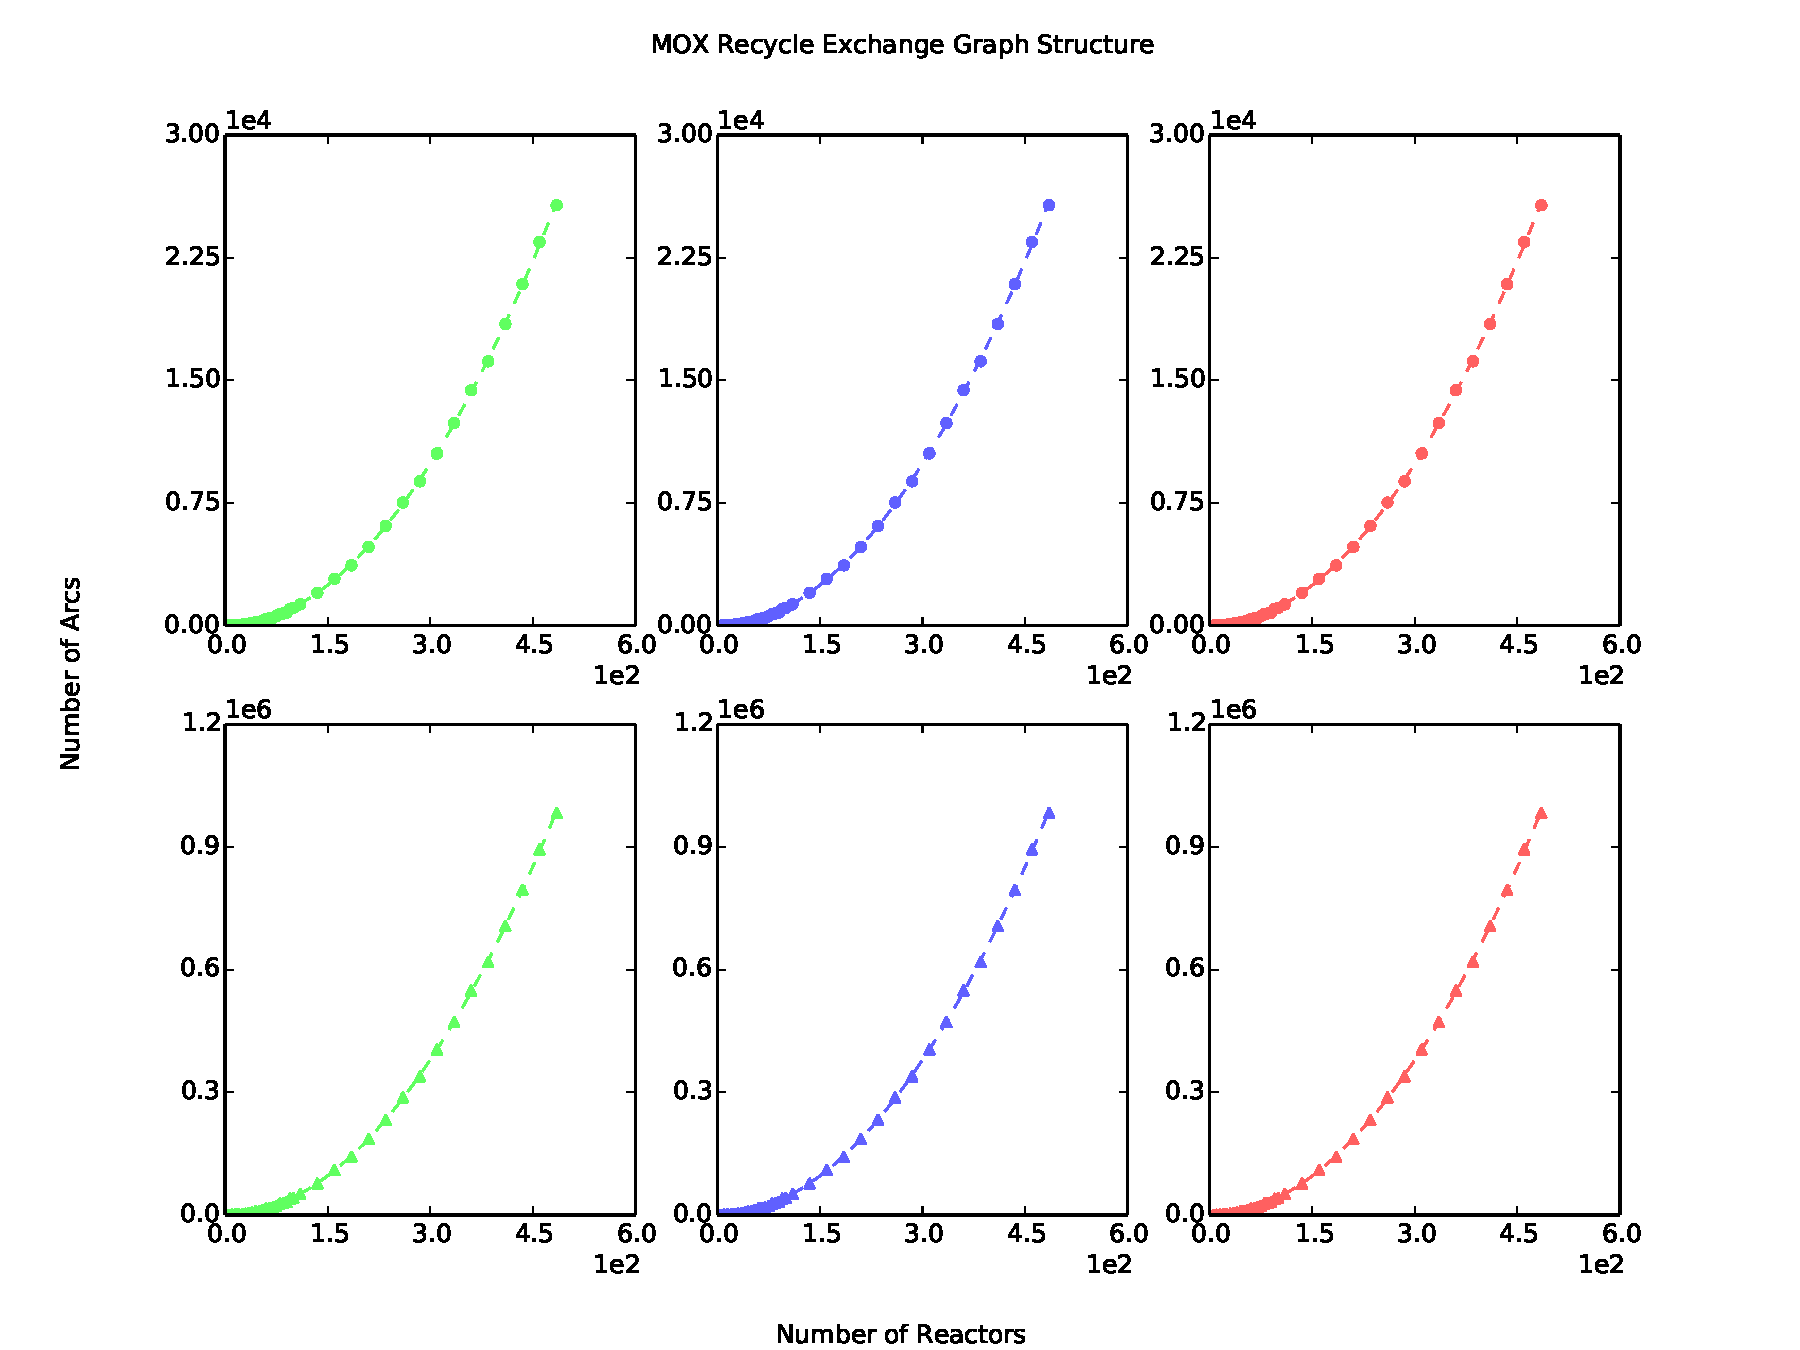
\includegraphics[width=.7\textwidth]{base_front_n_rxtr_n_arcs_fc1_solvergreedy.pdf}
    \caption[]{
      \label{fig:base_front_n_rxtr_n_arcs_fc1_solvergreedy}
      Arc population scaling with the number of reactors with coresponding linear fits.}
  \end{center}
\end{figure}

\begin{figure}[h!]
  \begin{center}
    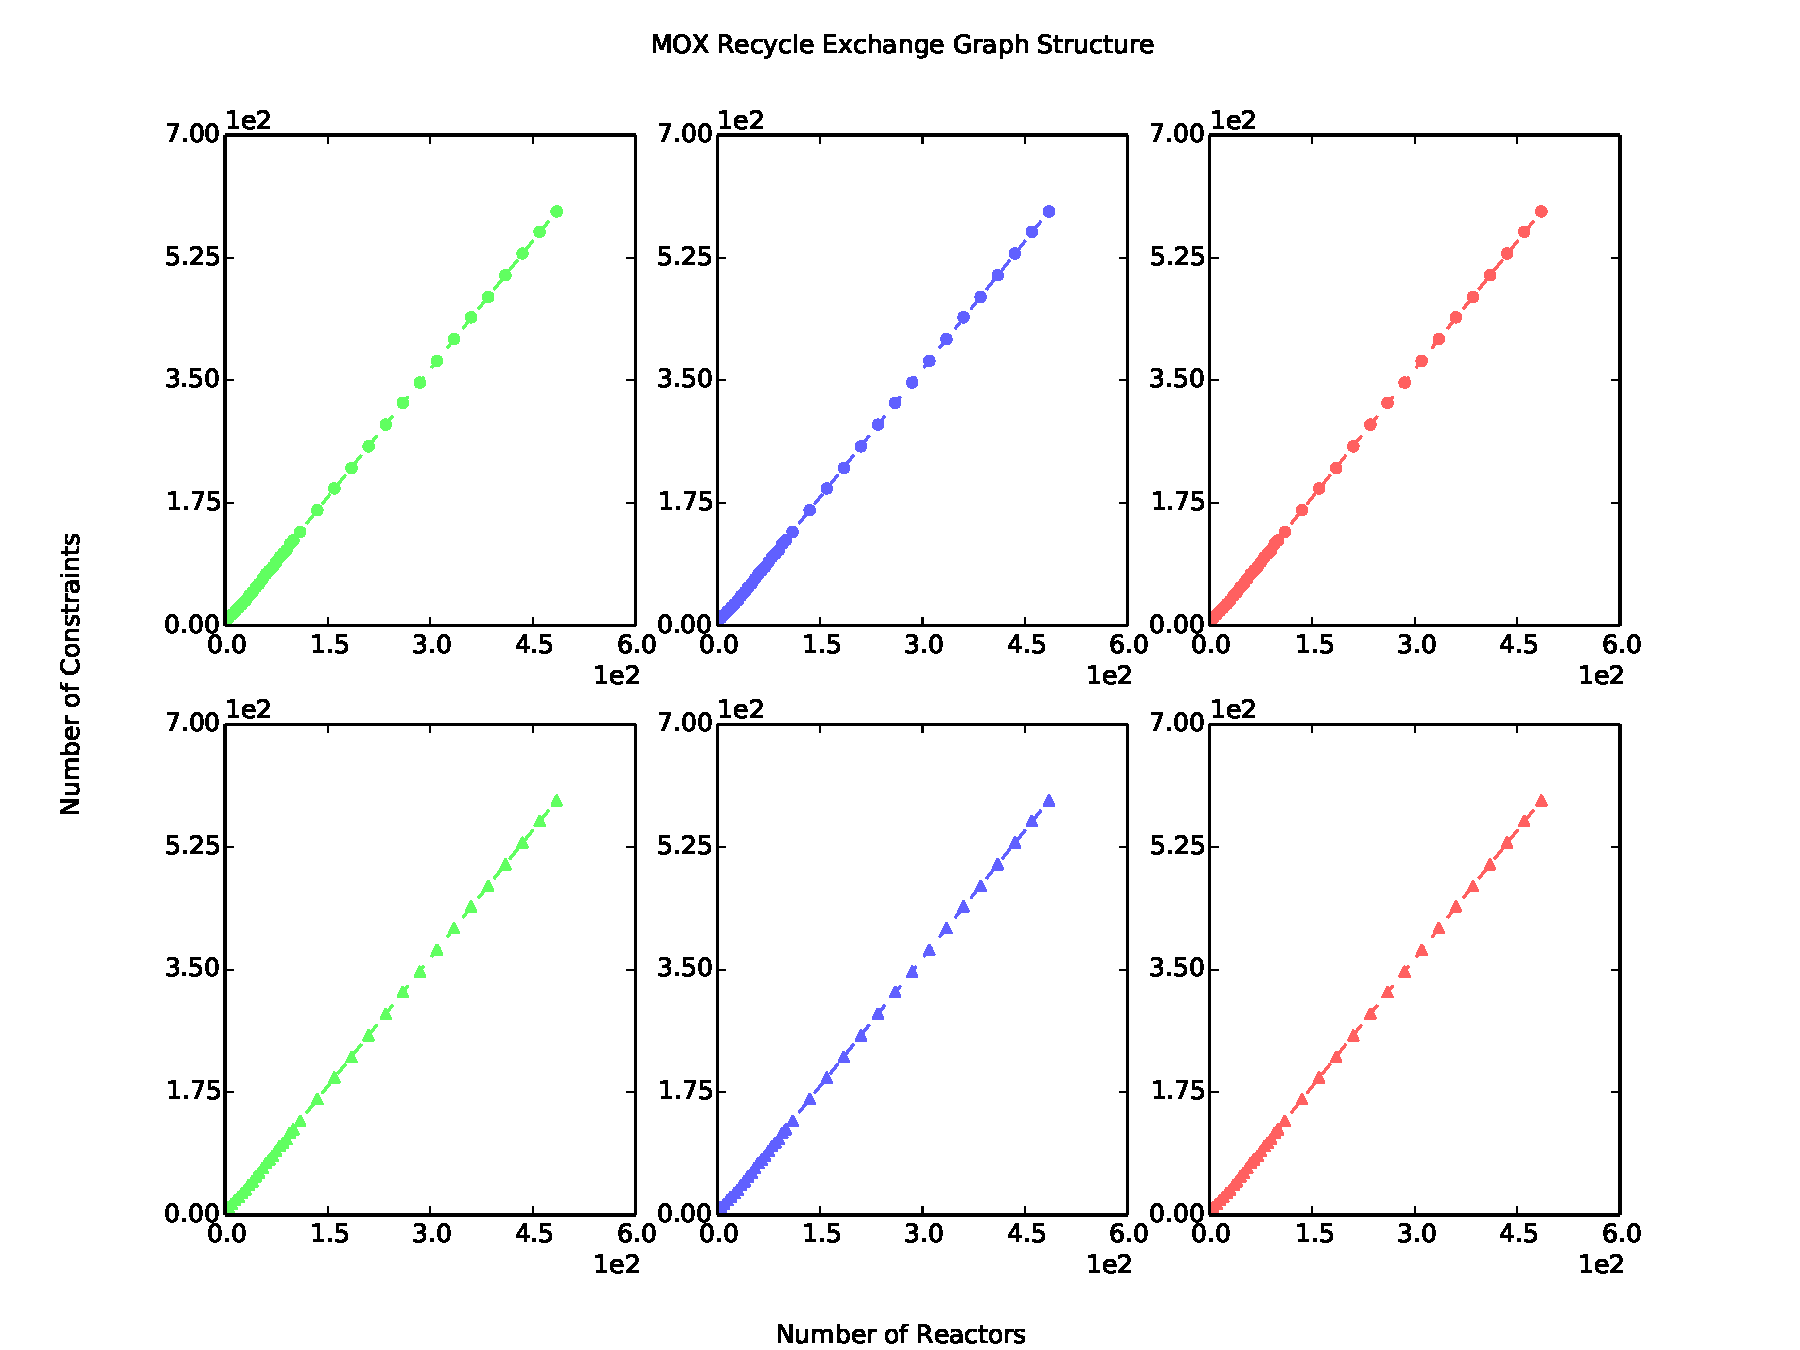
\includegraphics[width=.7\textwidth]{base_front_n_rxtr_n_constrs_fc1_solvergreedy.pdf}
    \caption[]{
      \label{fig:base_front_n_rxtr_n_constrs_fc1_solvergreedy}
      Constraint population scaling with the number of reactors with
      corresponding quadratic fits.}
  \end{center}
\end{figure}


\paragraph{Greedy Solver}

\cref{fig:base_front_n_rxtr_time_fc0_solvergreedy,fig:base_front_n_rxtr_time_fc1_solvergreedy,fig:base_front_n_rxtr_time_fc2_solvergreedy}
show the Greedy Solver results as the number of reactors increases for the OT,
MOX, and ThOX fuel cycles, respectively. Plotted with each data series is a
second-order polynomial fit, suggesting that the Greedy Solver scales as
$\mathcal{O}(n^2)$ in the number of reactors. As can be seen, this scaling is
independent of any fundamental parameter, as it is seen in every combination
thereof.

\begin{figure}[h!]
  \begin{center}
    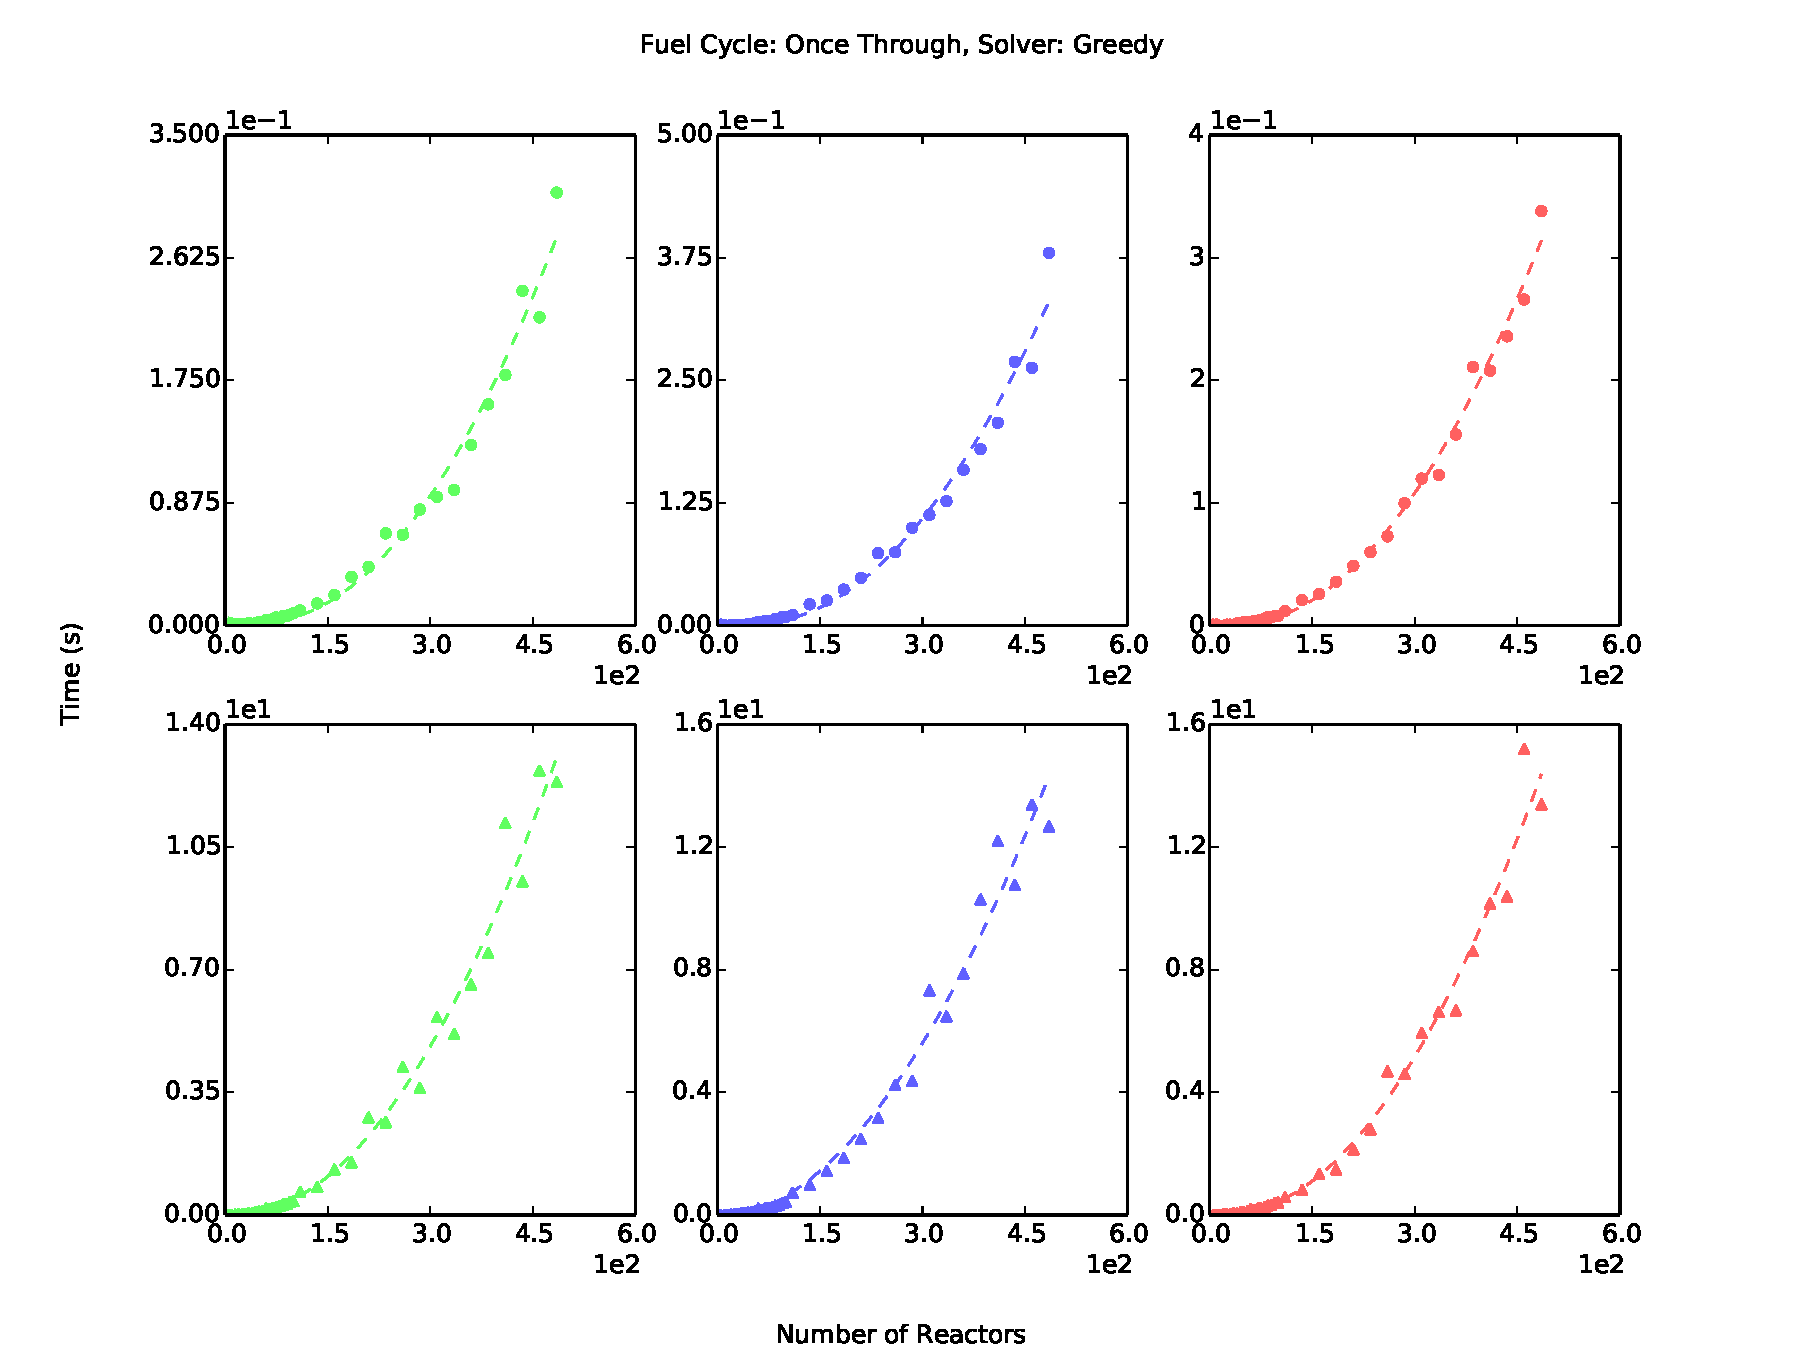
\includegraphics[width=.7\textwidth]{base_front_n_rxtr_time_fc0_solvergreedy.pdf}
    \caption[]{
      \label{fig:base_front_n_rxtr_time_fc0_solvergreedy}
      Greedy Solver results for the OT fuel cycle as the number of reactors
      increases.  }
  \end{center}
\end{figure}

\begin{figure}[h!]
  \begin{center}
    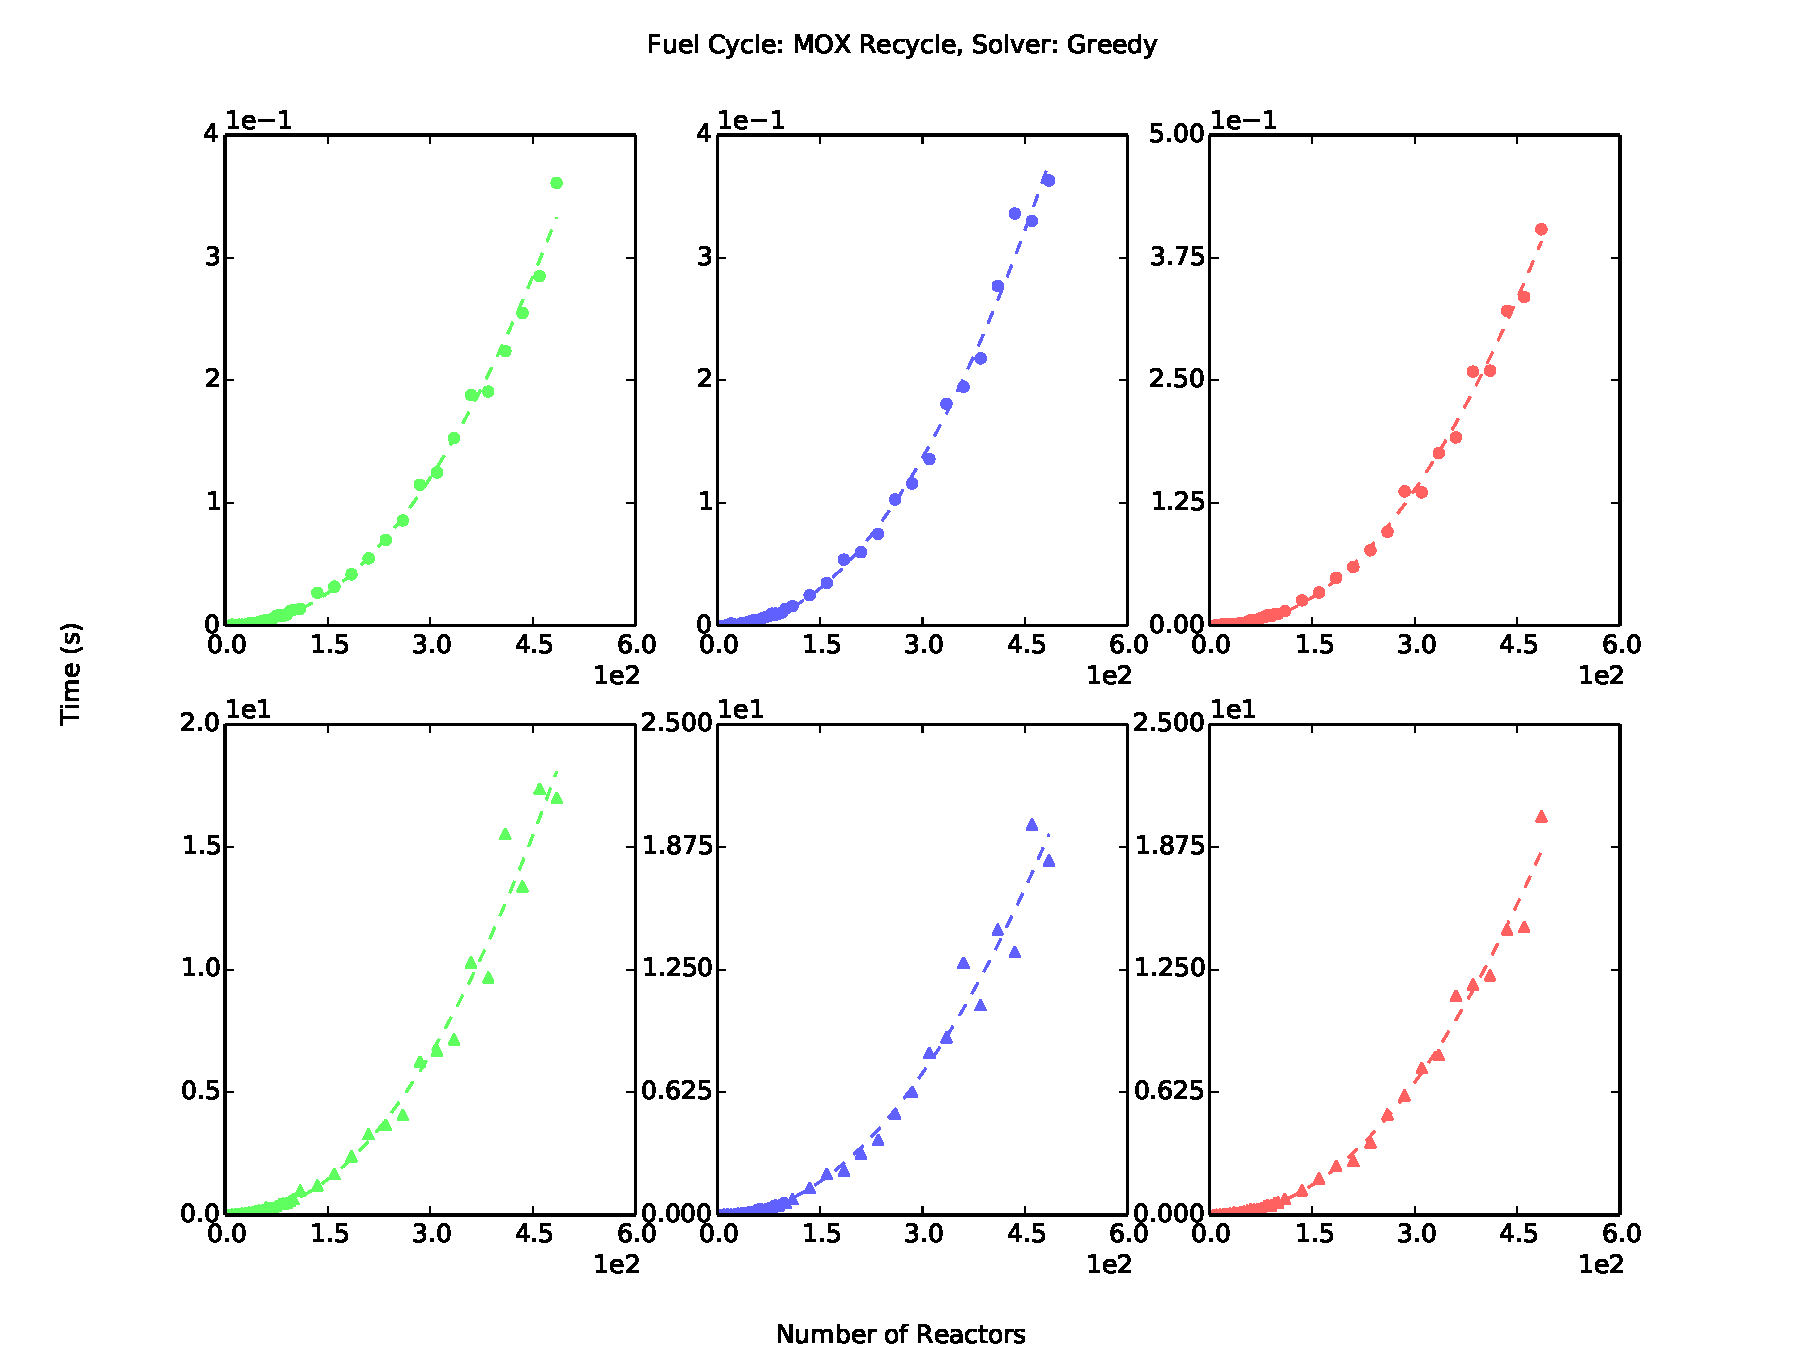
\includegraphics[width=.7\textwidth]{base_front_n_rxtr_time_fc1_solvergreedy.pdf}
    \caption[]{
      \label{fig:base_front_n_rxtr_time_fc1_solvergreedy}
      Greedy Solver results for the MOX fuel cycle as the number of reactors
      increases.
    }
  \end{center}
\end{figure}

\begin{figure}[h!]
  \begin{center}
    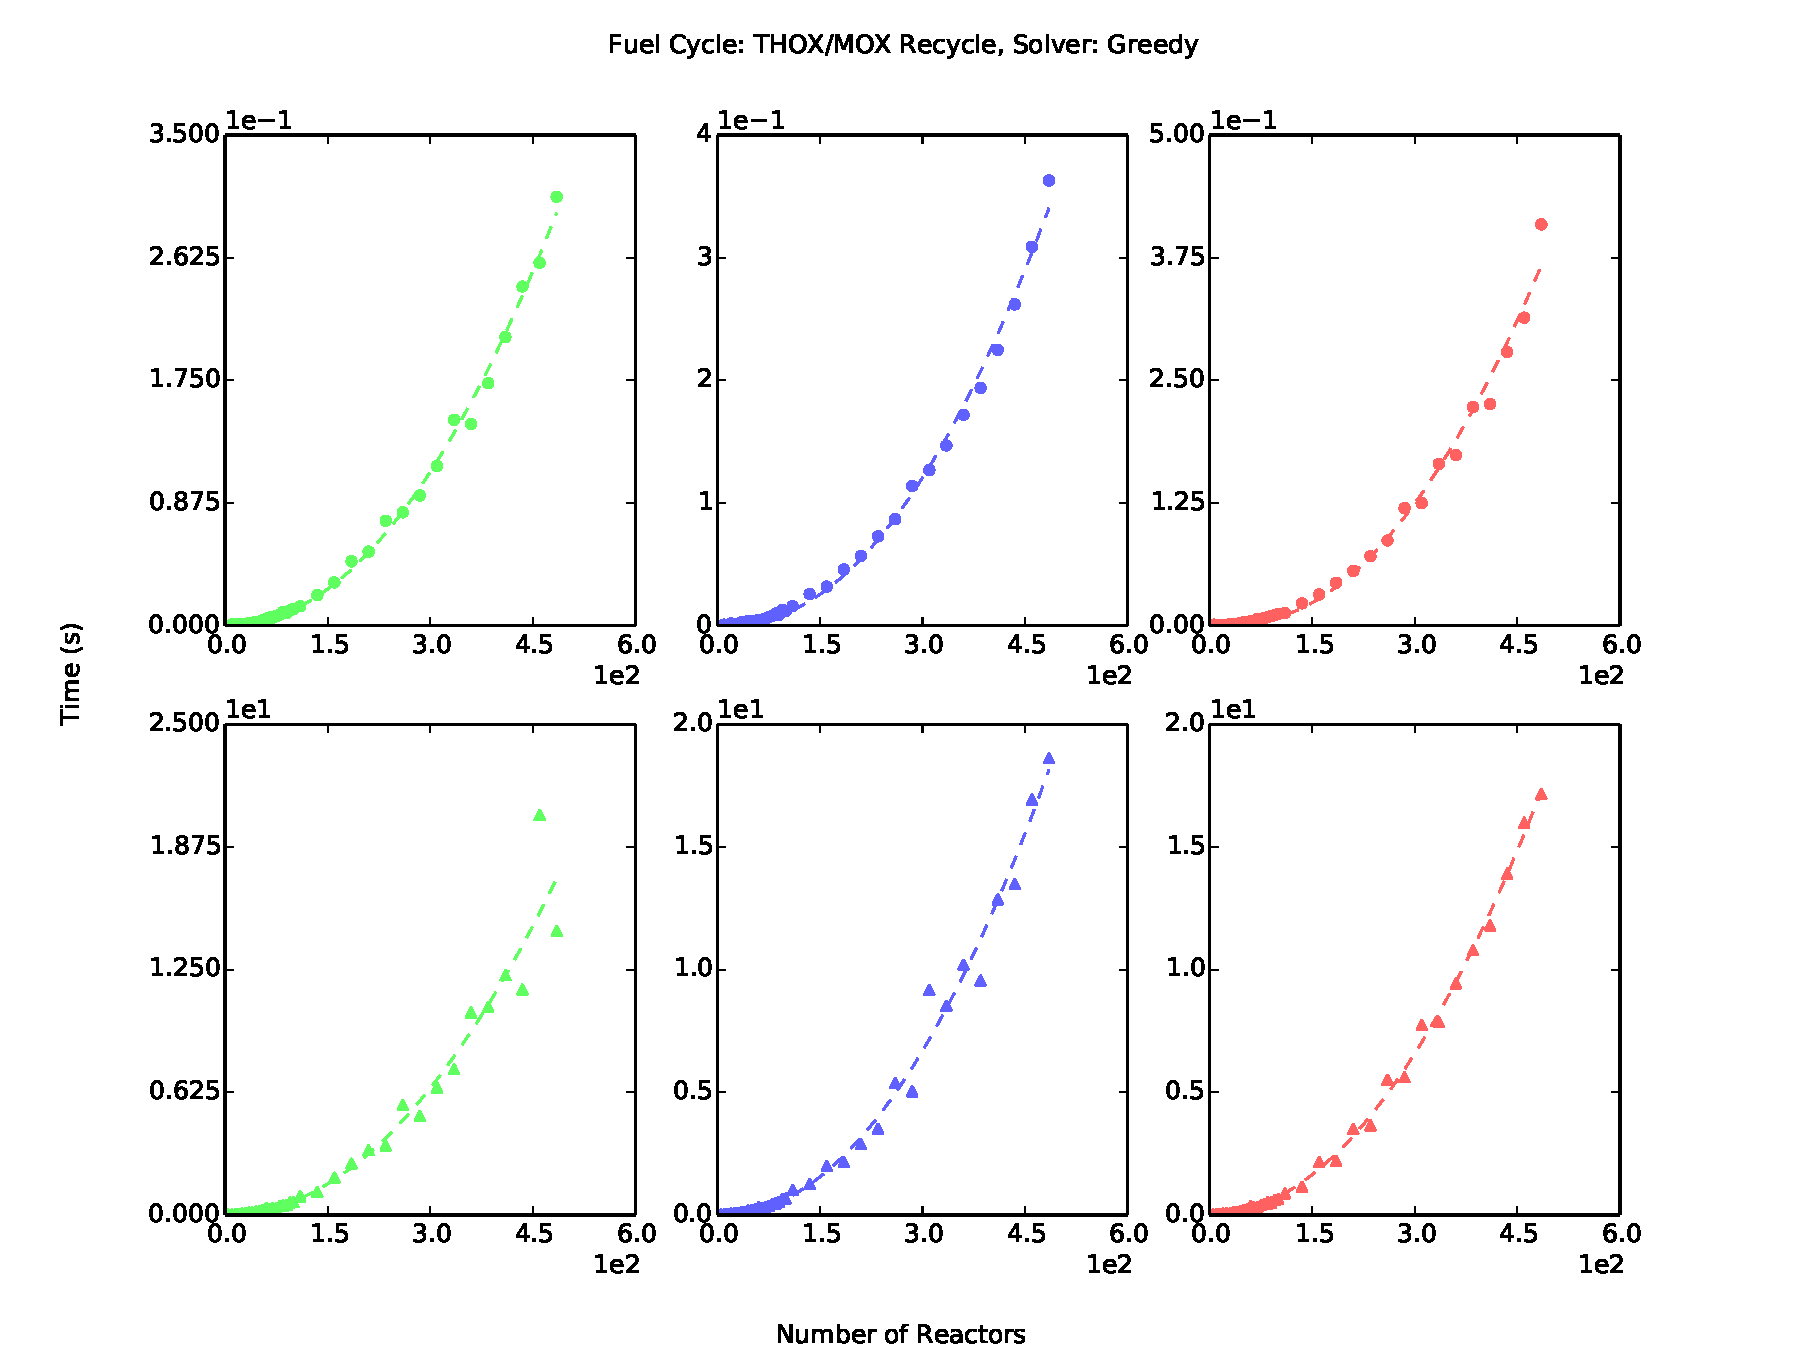
\includegraphics[width=.7\textwidth]{base_front_n_rxtr_time_fc2_solvergreedy.pdf}
    \caption[]{
      \label{fig:base_front_n_rxtr_time_fc2_solvergreedy}
      Greedy Solver results for the ThOX fuel cycle as the number of reactors
      increases.
      }
  \end{center}
\end{figure}

As was shown previously, the number of arcs in a generated exchange is an
$\mathcal{O}(n^2)$ effect. \ref{fig:base_front_n_arcs_time_fc1_solvergreedy}
graphs the same solution populations shown previously for the MOX fuel cycle as
a function of the number of arcs in the system. Plotted alongside the data are
linear curve fits. As can be seen, solution times scale linearly with the number
of arcs in the system. These trends are consistent across all three modeled fuel
cycles.

\begin{figure}[h!]
  \begin{center}
    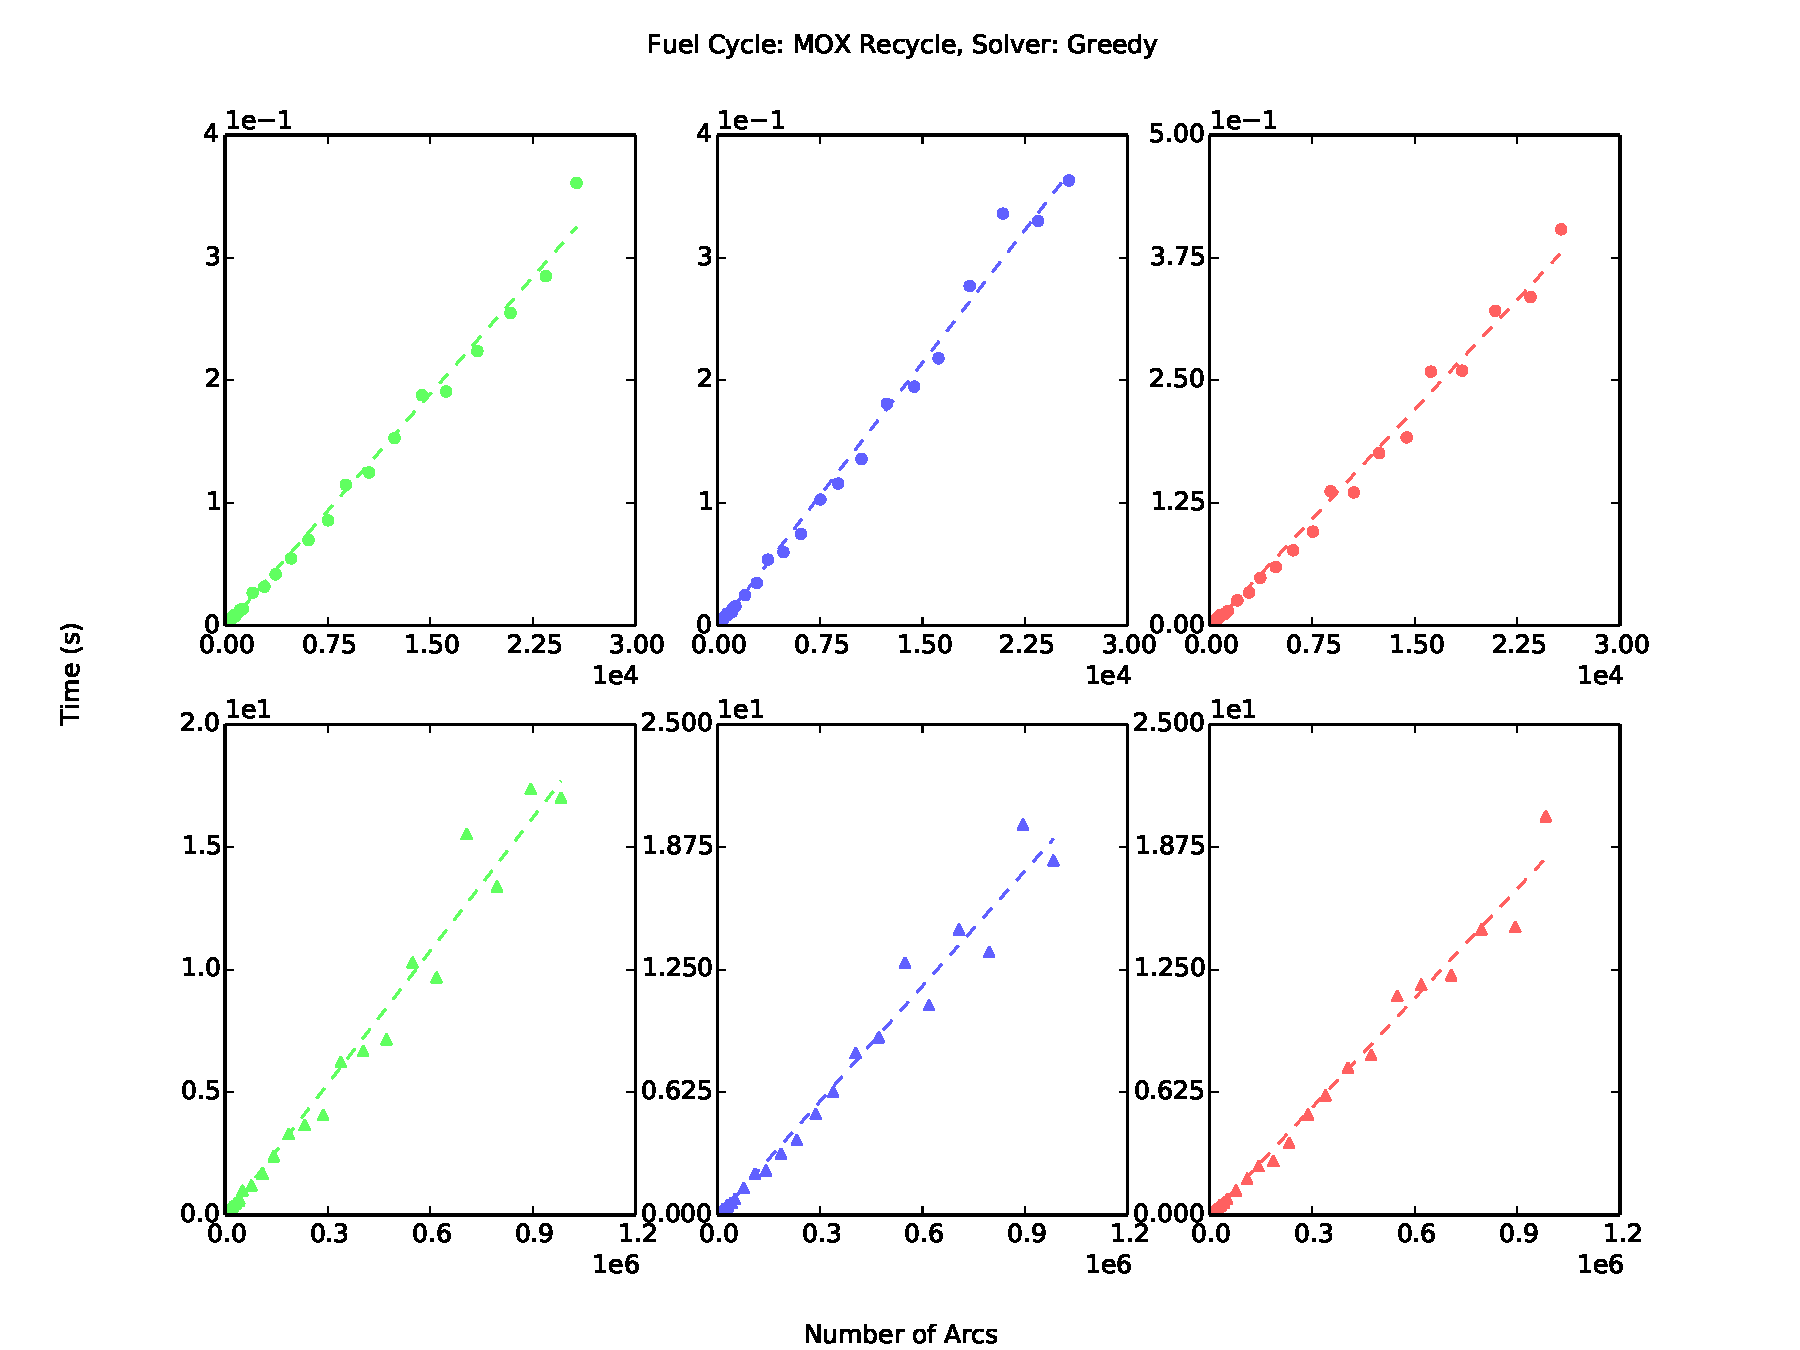
\includegraphics[width=.7\textwidth]{base_front_n_arcs_time_fc1_solvergreedy.pdf}
    \caption[]{
      \label{fig:base_front_n_arcs_time_fc1_solvergreedy}
      Greedy Solver results for the MOX fuel cycle as the number of arcs
      increases.      
    }
  \end{center}
\end{figure}

\paragraph{CLP Solver}

Interestingly, the CLP solver shows the same scaling behavior as the Greedy
Solver, and that behavior is also independent of fundamental parameter. The
number of arcs in the system drives the solution time scaling, as can be seen in
\Cref{fig:base_front_n_arcs_time_fc0_solverclp,fig:base_front_n_arcs_time_fc1_solverclp,fig:base_front_n_arcs_time_fc2_solverclp}.

\begin{figure}[h!]
  \begin{center}
    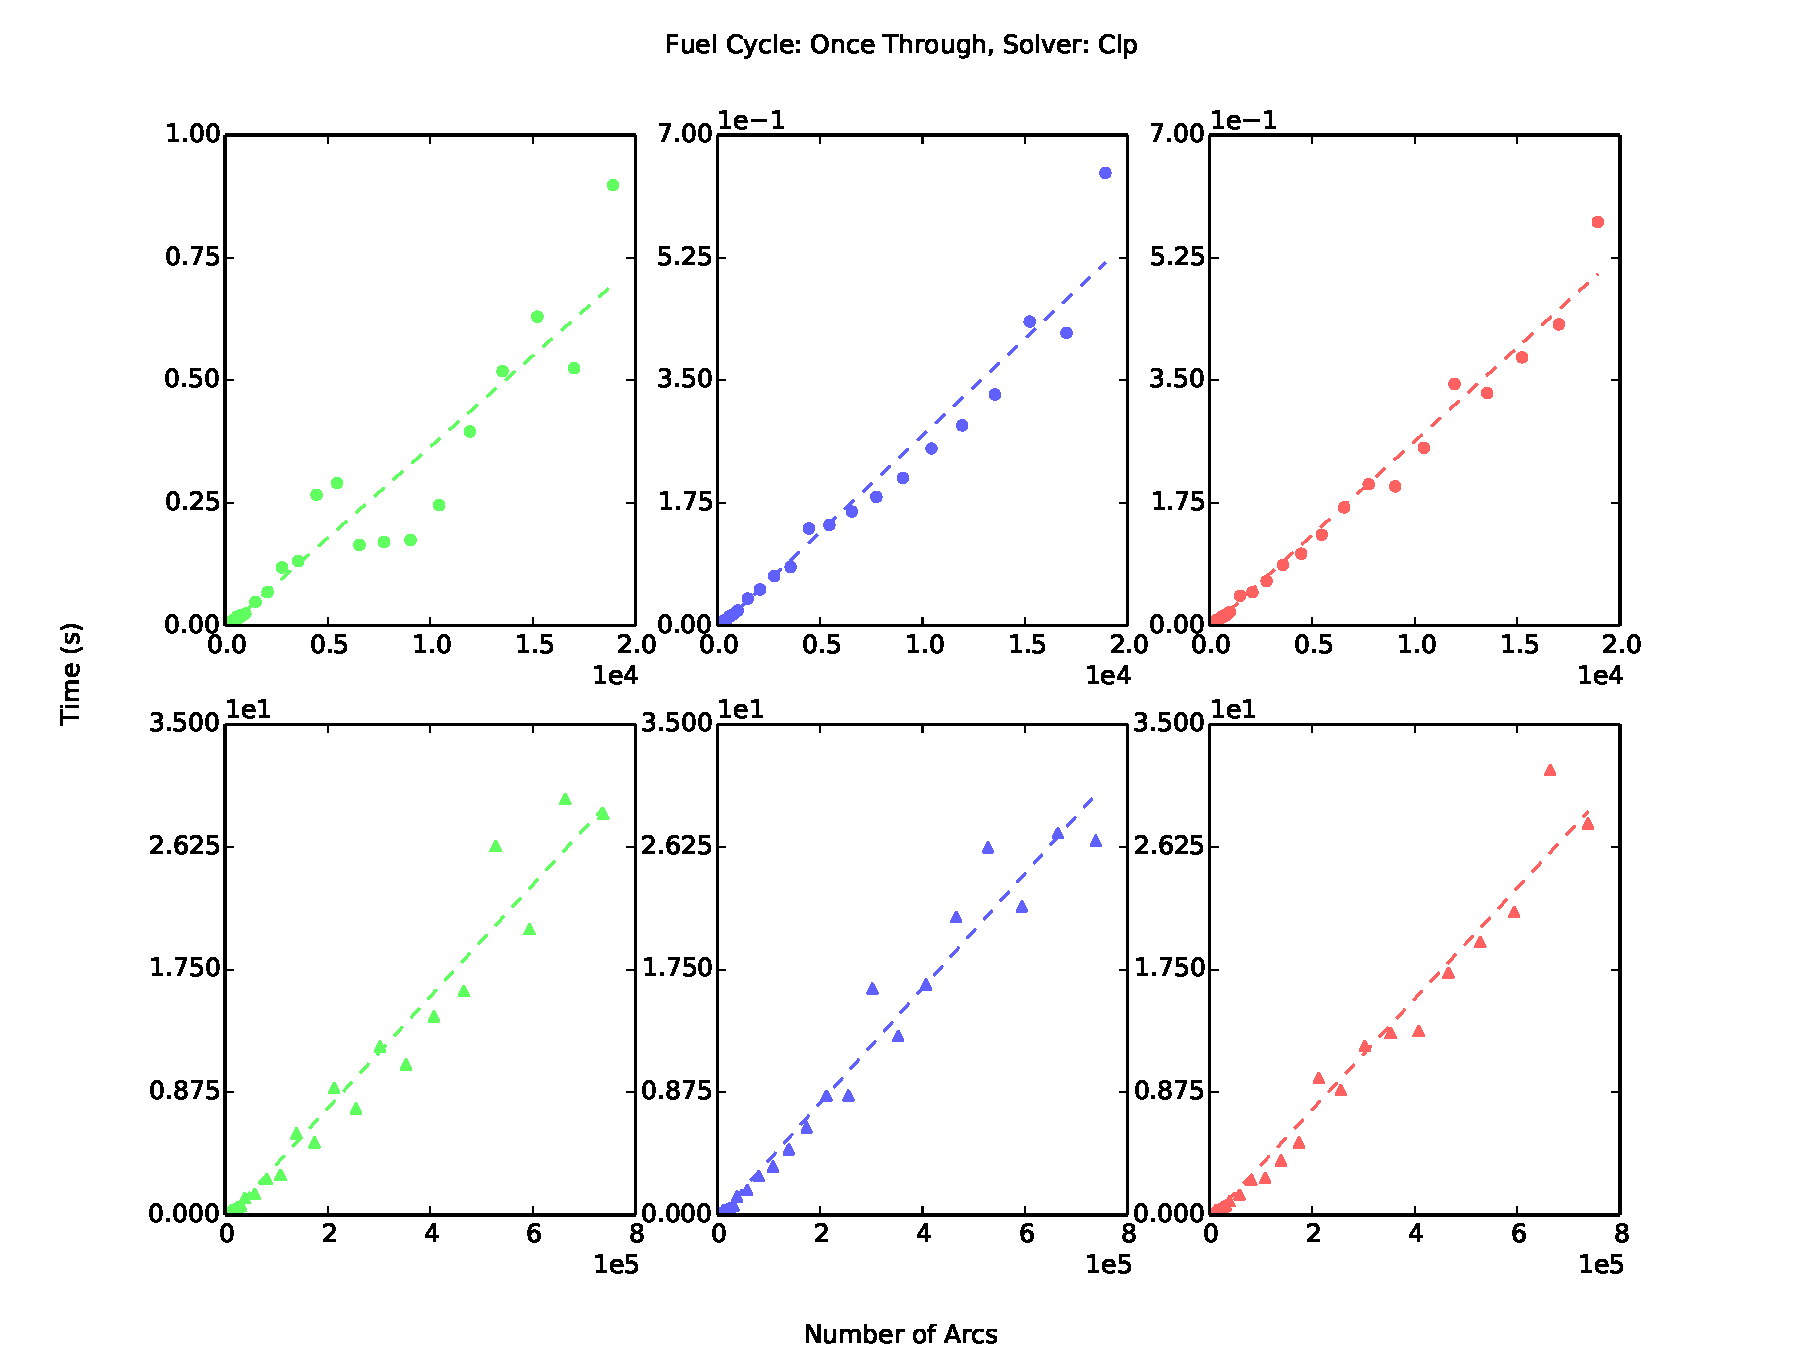
\includegraphics[width=.7\textwidth]{base_front_n_arcs_time_fc0_solverclp.pdf}
    \caption[]{
      \label{fig:base_front_n_arcs_time_fc0_solverclp}
      CLP Solver results for the OT fuel cycle as the number of arcs
      increases.
      }
  \end{center}
\end{figure}

\begin{figure}[h!]
  \begin{center}
    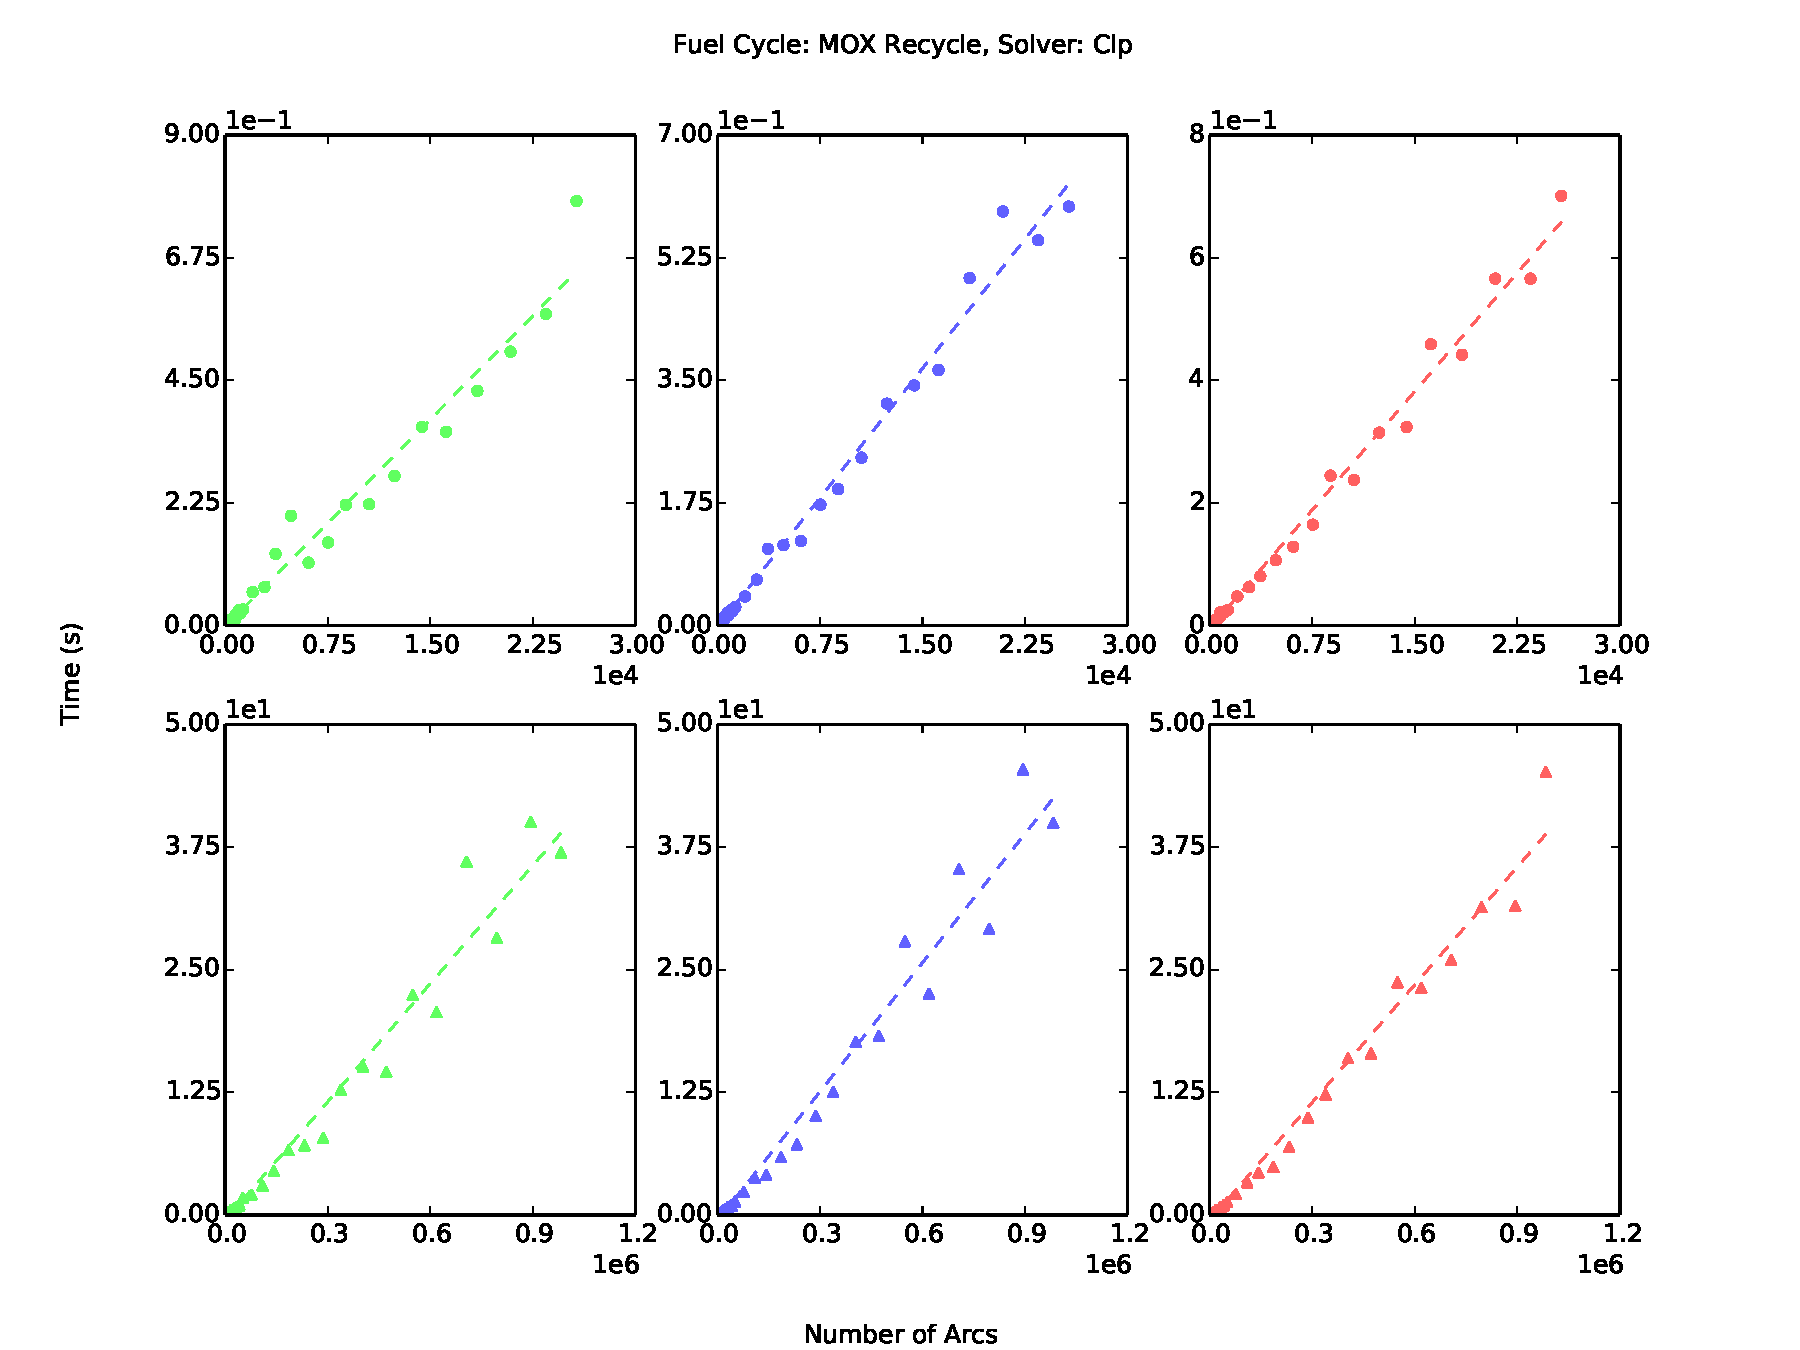
\includegraphics[width=.7\textwidth]{base_front_n_arcs_time_fc1_solverclp.pdf}
    \caption[]{
      \label{fig:base_front_n_arcs_time_fc1_solverclp}
      CLP Solver results for the MOX fuel cycle as the number of arcs
      increases.
      }
  \end{center}
\end{figure}

\begin{figure}[h!]
  \begin{center}
    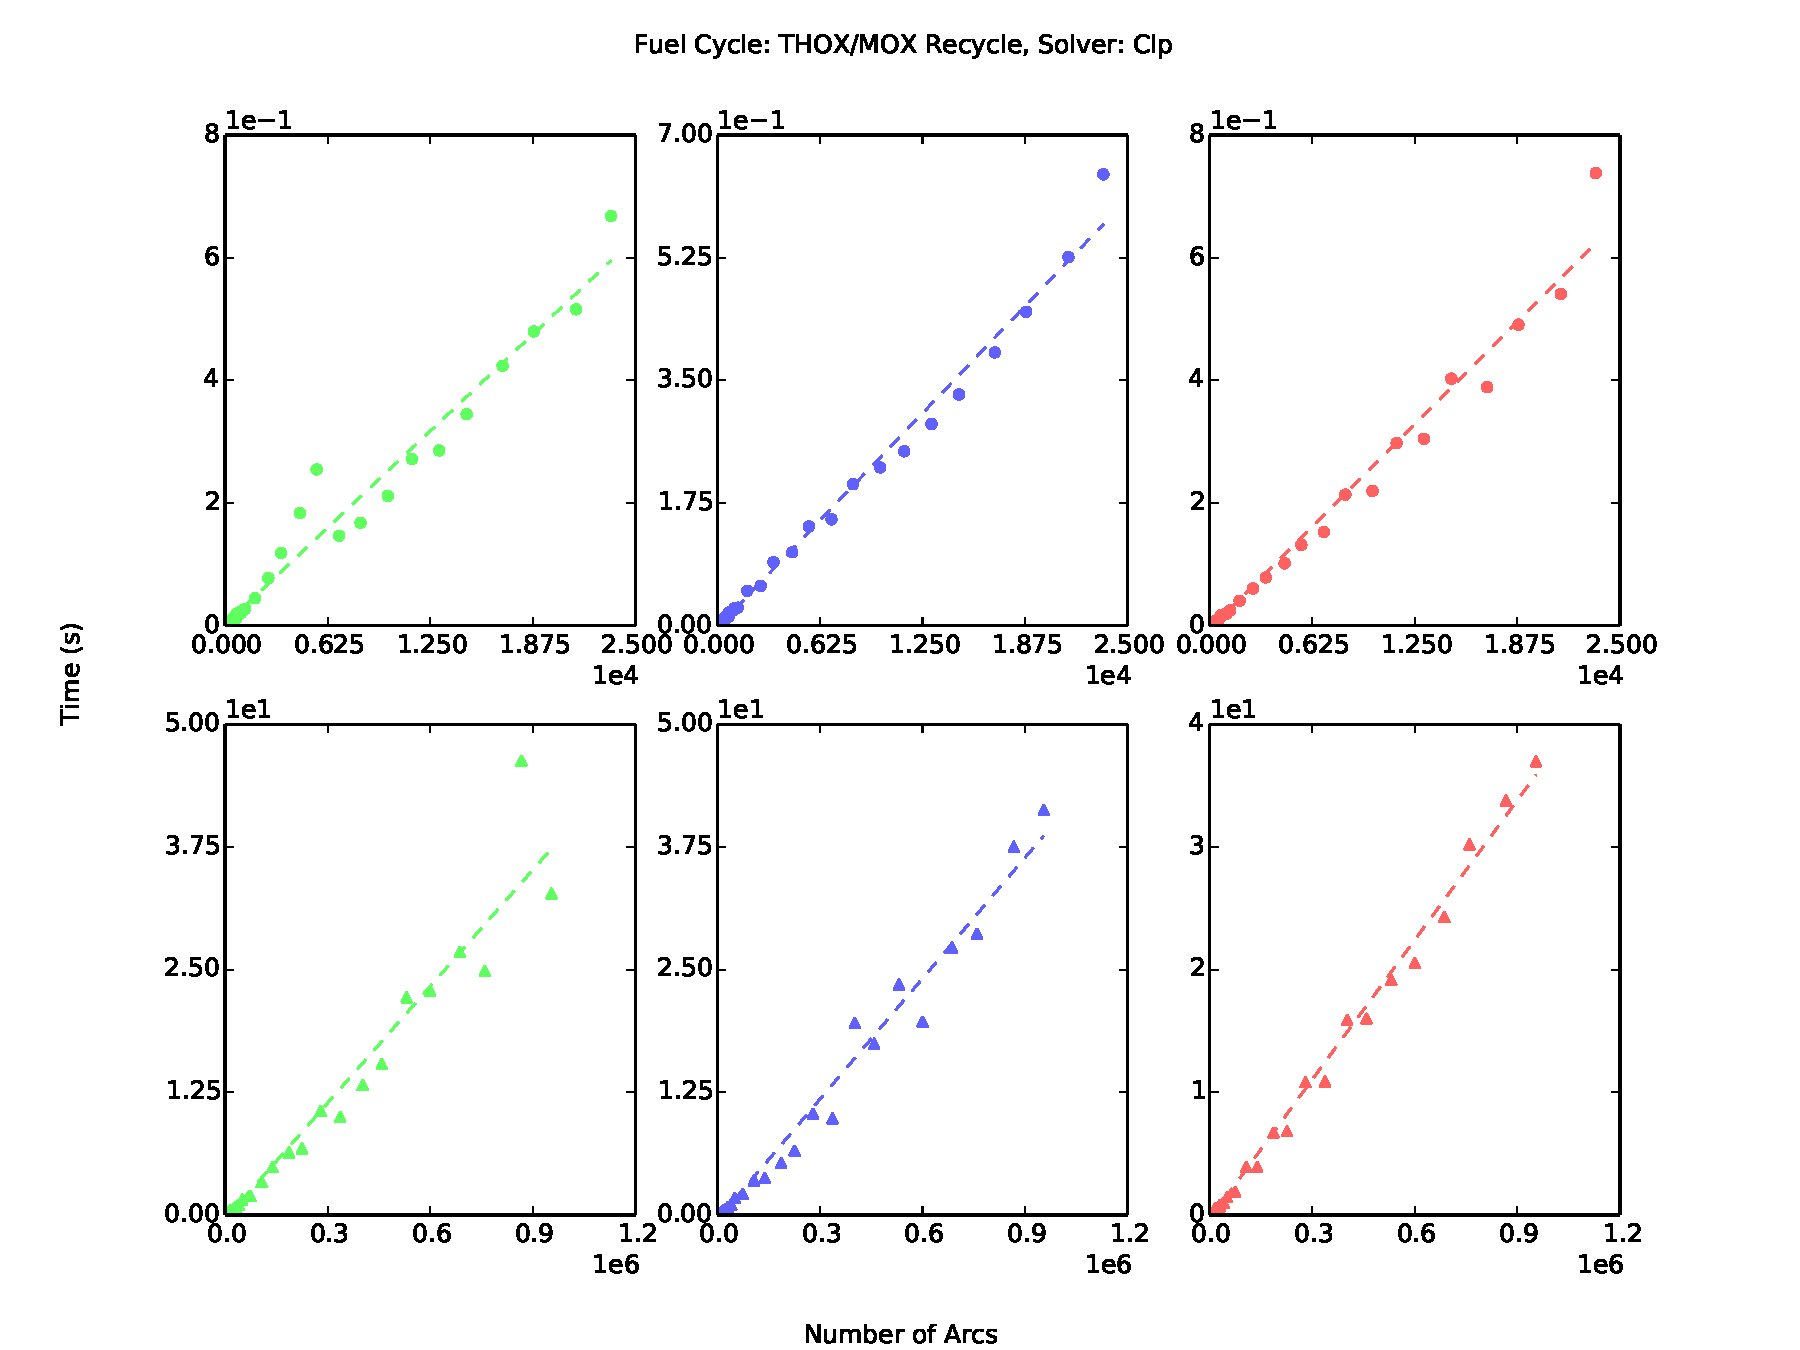
\includegraphics[width=.7\textwidth]{base_front_n_arcs_time_fc2_solverclp.pdf}
    \caption[]{
      \label{fig:base_front_n_arcs_time_fc2_solverclp}
      CLP Solver results for the ThOX fuel cycle as the number of arcs
      increases.
      }
  \end{center}
\end{figure}

\paragraph{CBC Solver}

The CBC solver is much more sporadic than either the CLP or Greedy solvers, as
is expected, for MILP optimization problems are NP-Hard. An artificial, 3-hour
time limit was provided for CBC-solved instances, and a 1\% ratio-gap
convergence criteria was applied. In each of the figures below, only instances
reaching convergence are displayed in order to attempt to ascertain any related
trends. \Cref{fig:base_front_n_rxtr_time_fc0_solvercbc,fig:base_front_n_rxtr_time_fc1_solvercbc,fig:base_front_n_rxtr_time_fc2_solvercbc}
show timing results as a function of the number of reactors in the
system. \Cref{fig:base_front_n_arcs_time_fc0_solvercbc,fig:base_front_n_arcs_time_fc1_solvercbc,fig:base_front_n_arcs_time_fc2_solvercbc}
show timing results as a function of the number of arcs in the system. Note that
in each case below, a log-lin graph is used.

\begin{figure}[h!]
  \begin{center}
    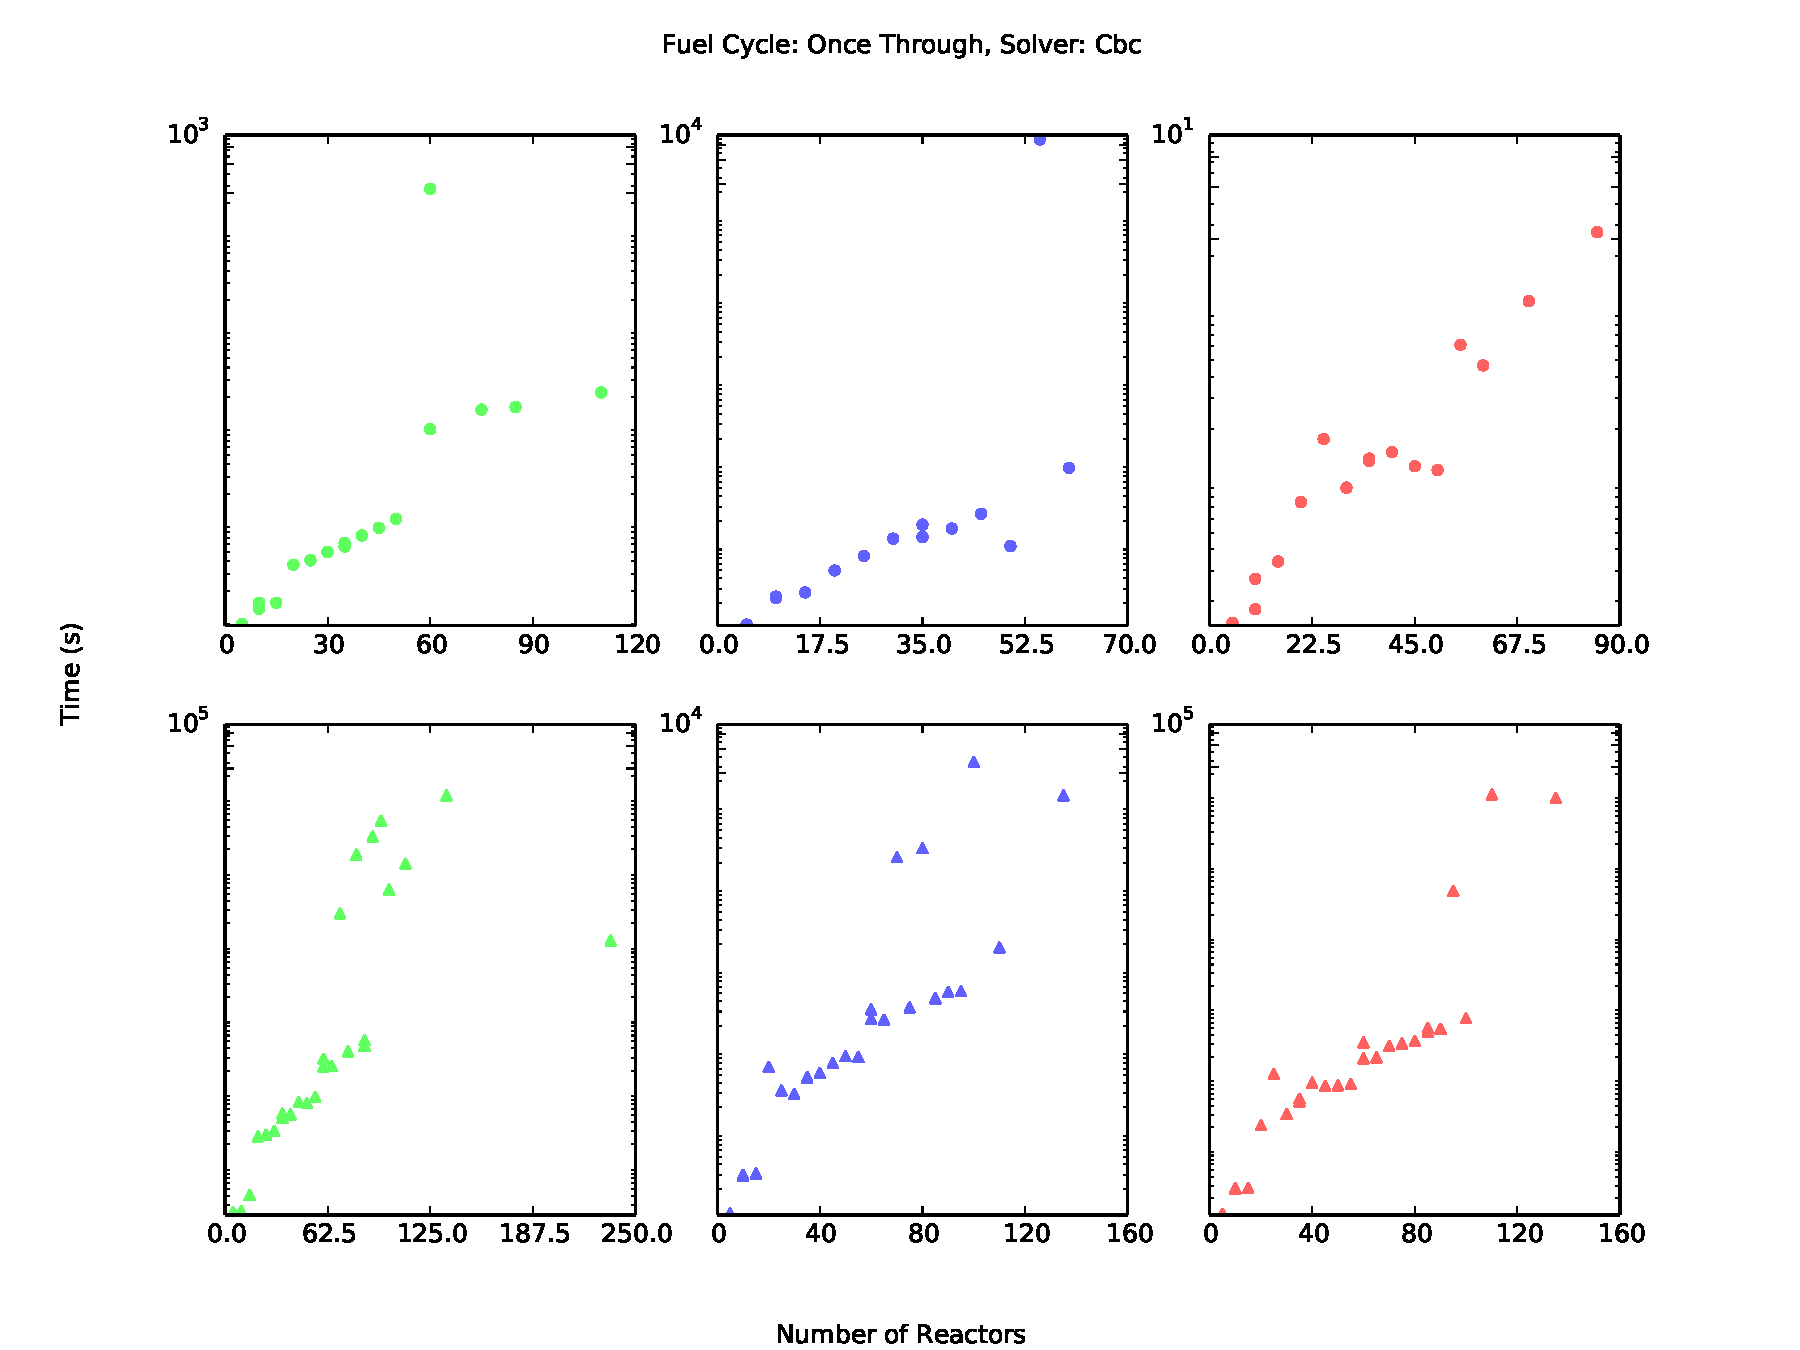
\includegraphics[width=.7\textwidth]{base_front_n_rxtr_time_fc0_solvercbc.pdf}
    \caption[]{
      \label{fig:base_front_n_rxtr_time_fc0_solvercbc}
      CBC Solver results for the OT fuel cycle as the number of reactors
      increases.
      }
  \end{center}
\end{figure}

\begin{figure}[h!]
  \begin{center}
    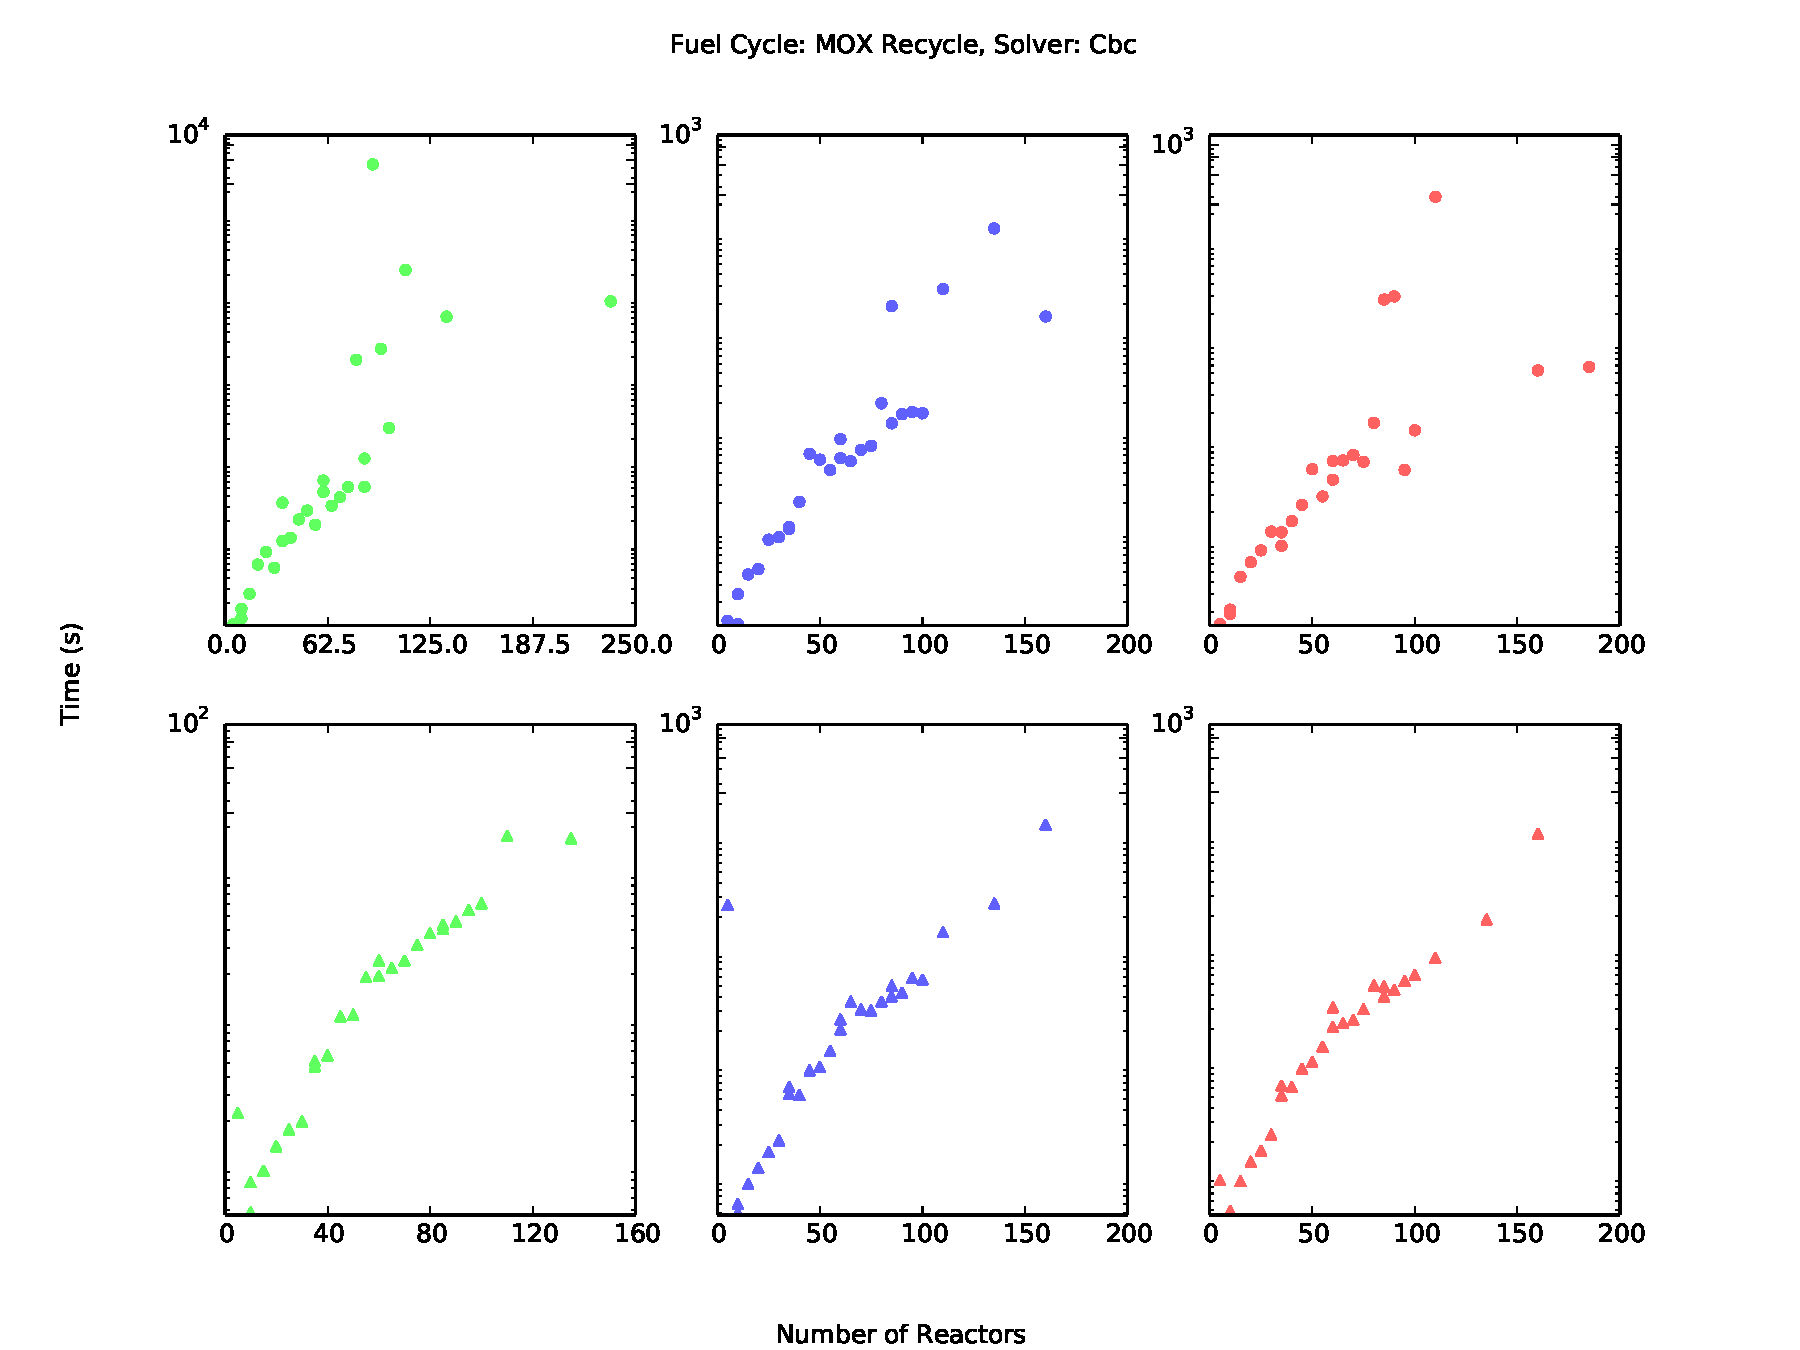
\includegraphics[width=.7\textwidth]{base_front_n_rxtr_time_fc1_solvercbc.pdf}
    \caption[]{
      \label{fig:base_front_n_rxtr_time_fc1_solvercbc}
      CBC Solver results for the MOX fuel cycle as the number of reactors
      increases.
      }
  \end{center}
\end{figure}

\begin{figure}[h!]
  \begin{center}
    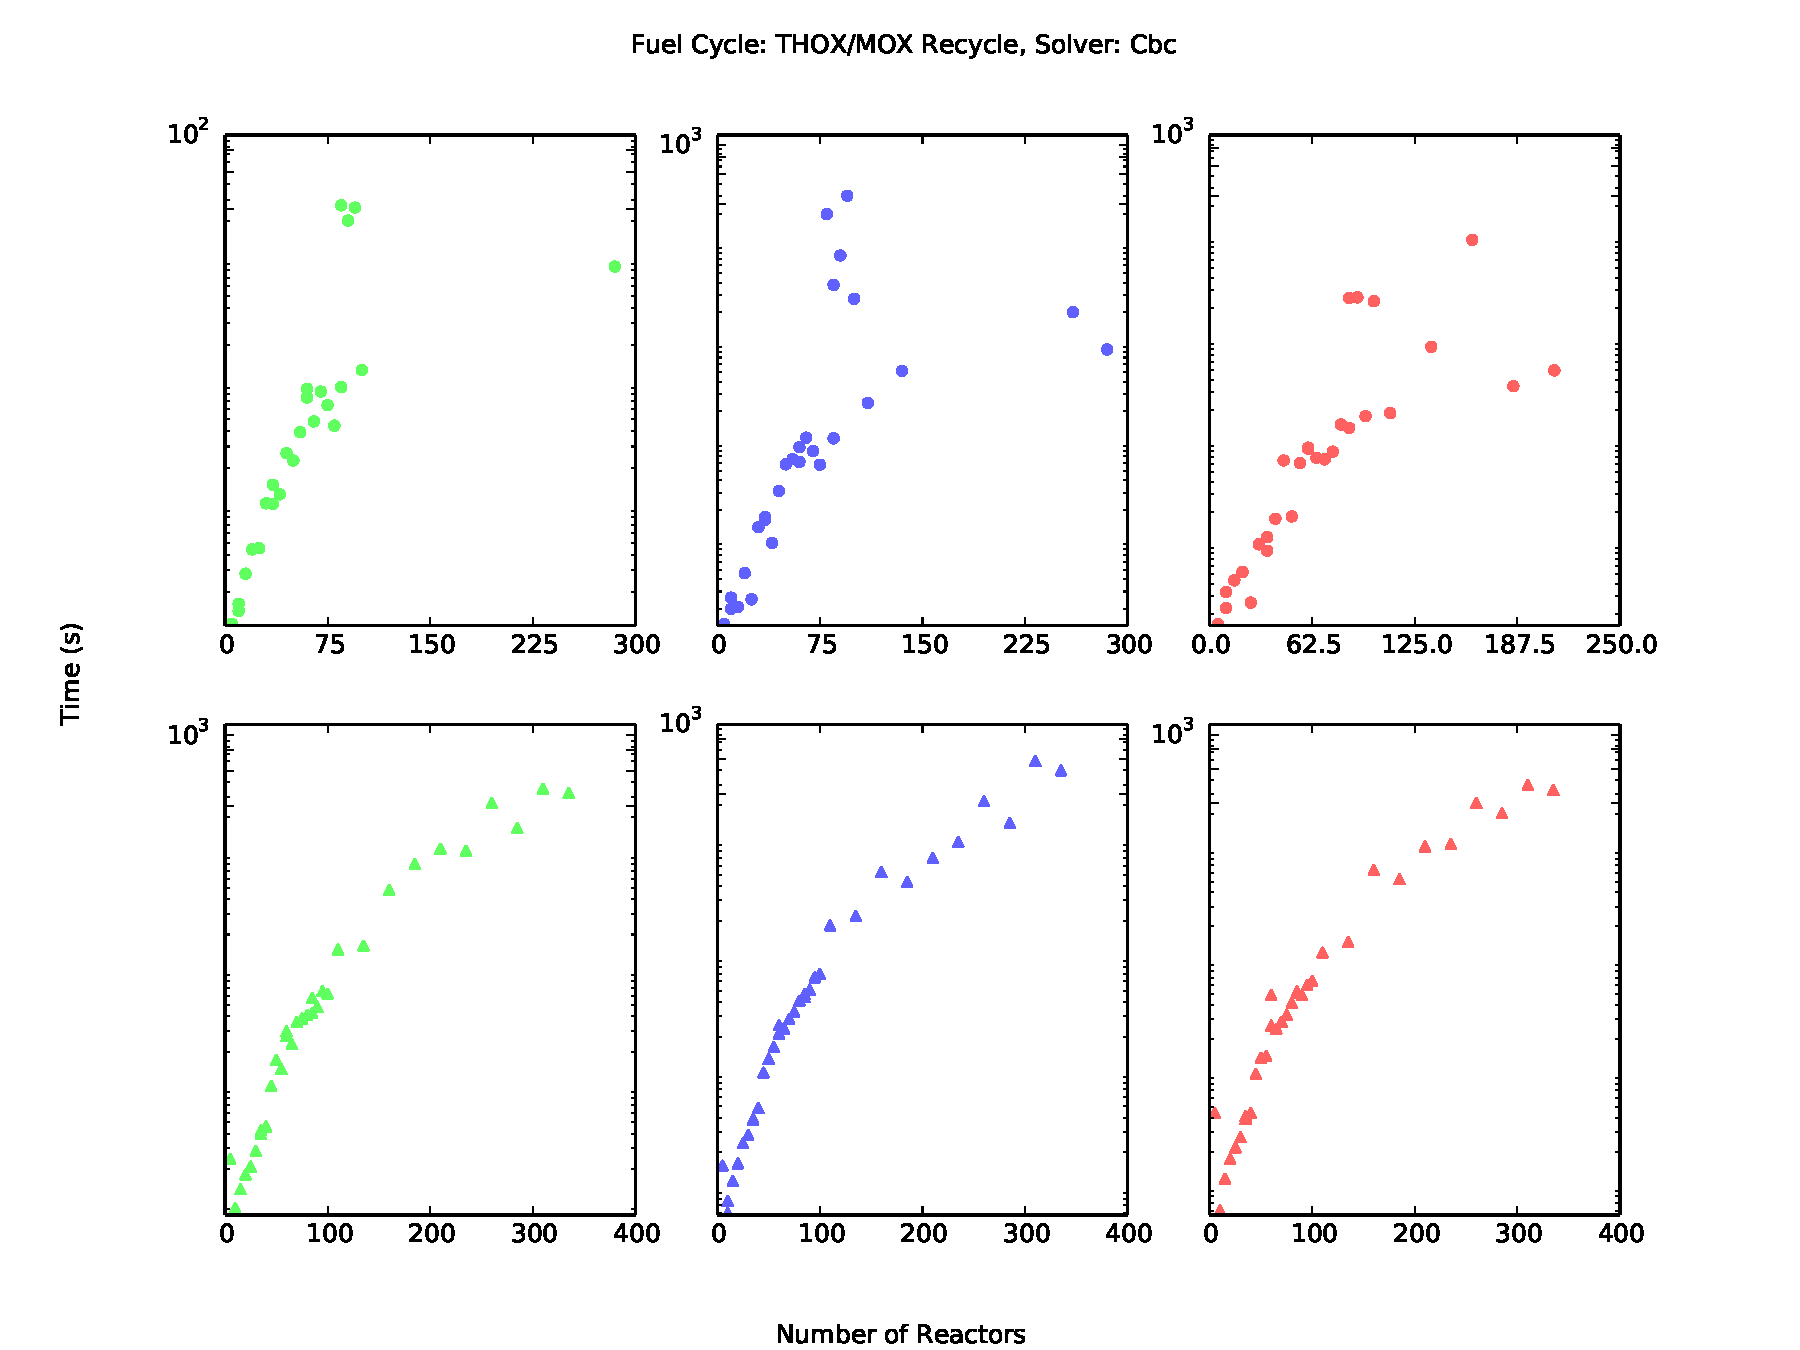
\includegraphics[width=.7\textwidth]{base_front_n_rxtr_time_fc2_solvercbc.pdf}
    \caption[]{
      \label{fig:base_front_n_rxtr_time_fc2_solvercbc}
      CBC Solver results for the ThOX fuel cycle as the number of reactors
      increases.
      }
  \end{center}
\end{figure}

\begin{figure}[h!]
  \begin{center}
    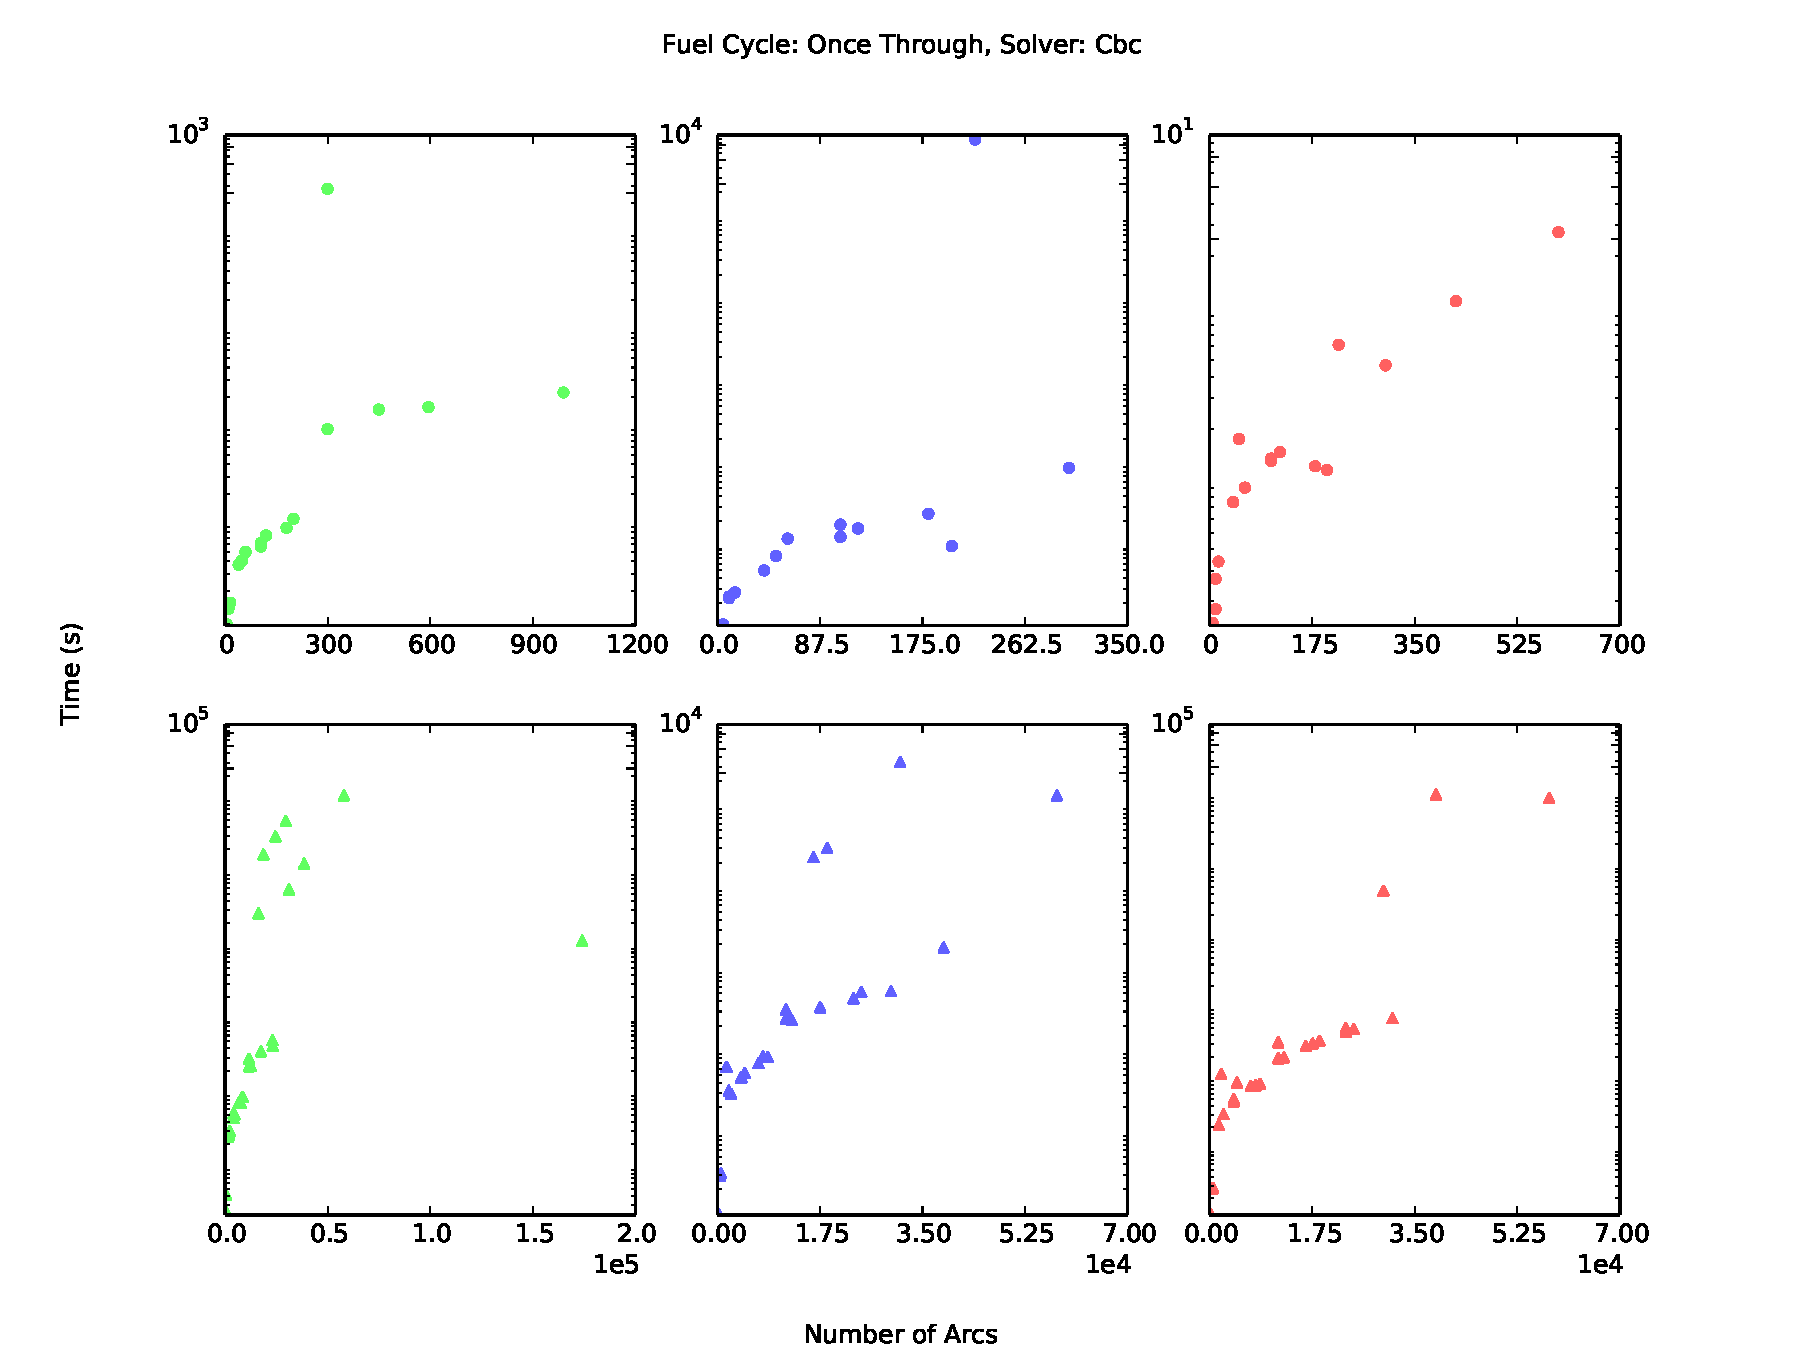
\includegraphics[width=.7\textwidth]{base_front_n_arcs_time_fc0_solvercbc.pdf}
    \caption[]{
      \label{fig:base_front_n_arcs_time_fc0_solvercbc}
      CBC Solver results for the OT fuel cycle as the number of arcs
      increases.
      }
  \end{center}
\end{figure}

\begin{figure}[h!]
  \begin{center}
    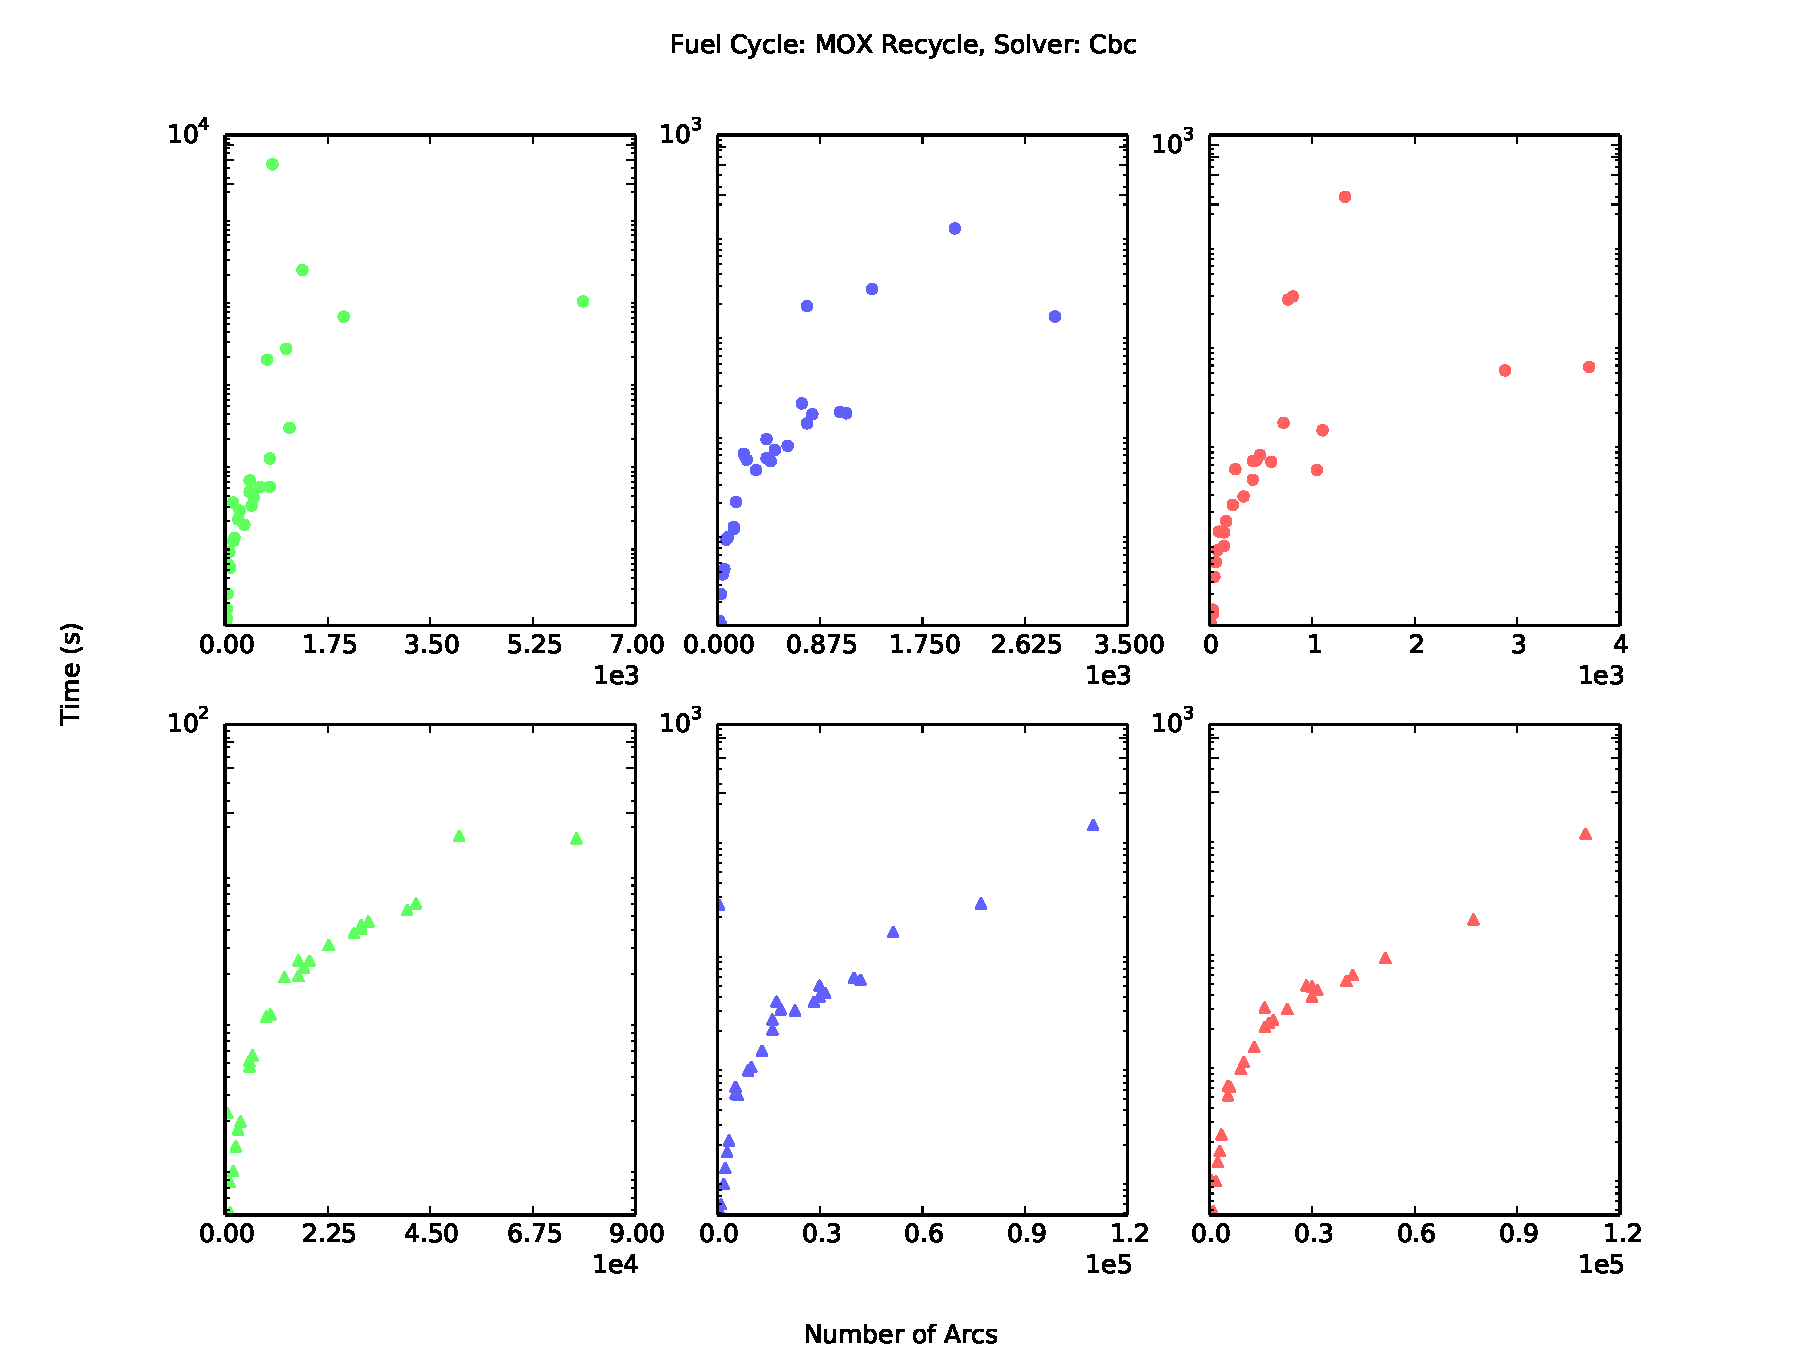
\includegraphics[width=.7\textwidth]{base_front_n_arcs_time_fc1_solvercbc.pdf}
    \caption[]{
      \label{fig:base_front_n_arcs_time_fc1_solvercbc}
      CBC Solver results for the MOX fuel cycle as the number of arcs
      increases.
      }
  \end{center}
\end{figure}

\begin{figure}[h!]
  \begin{center}
    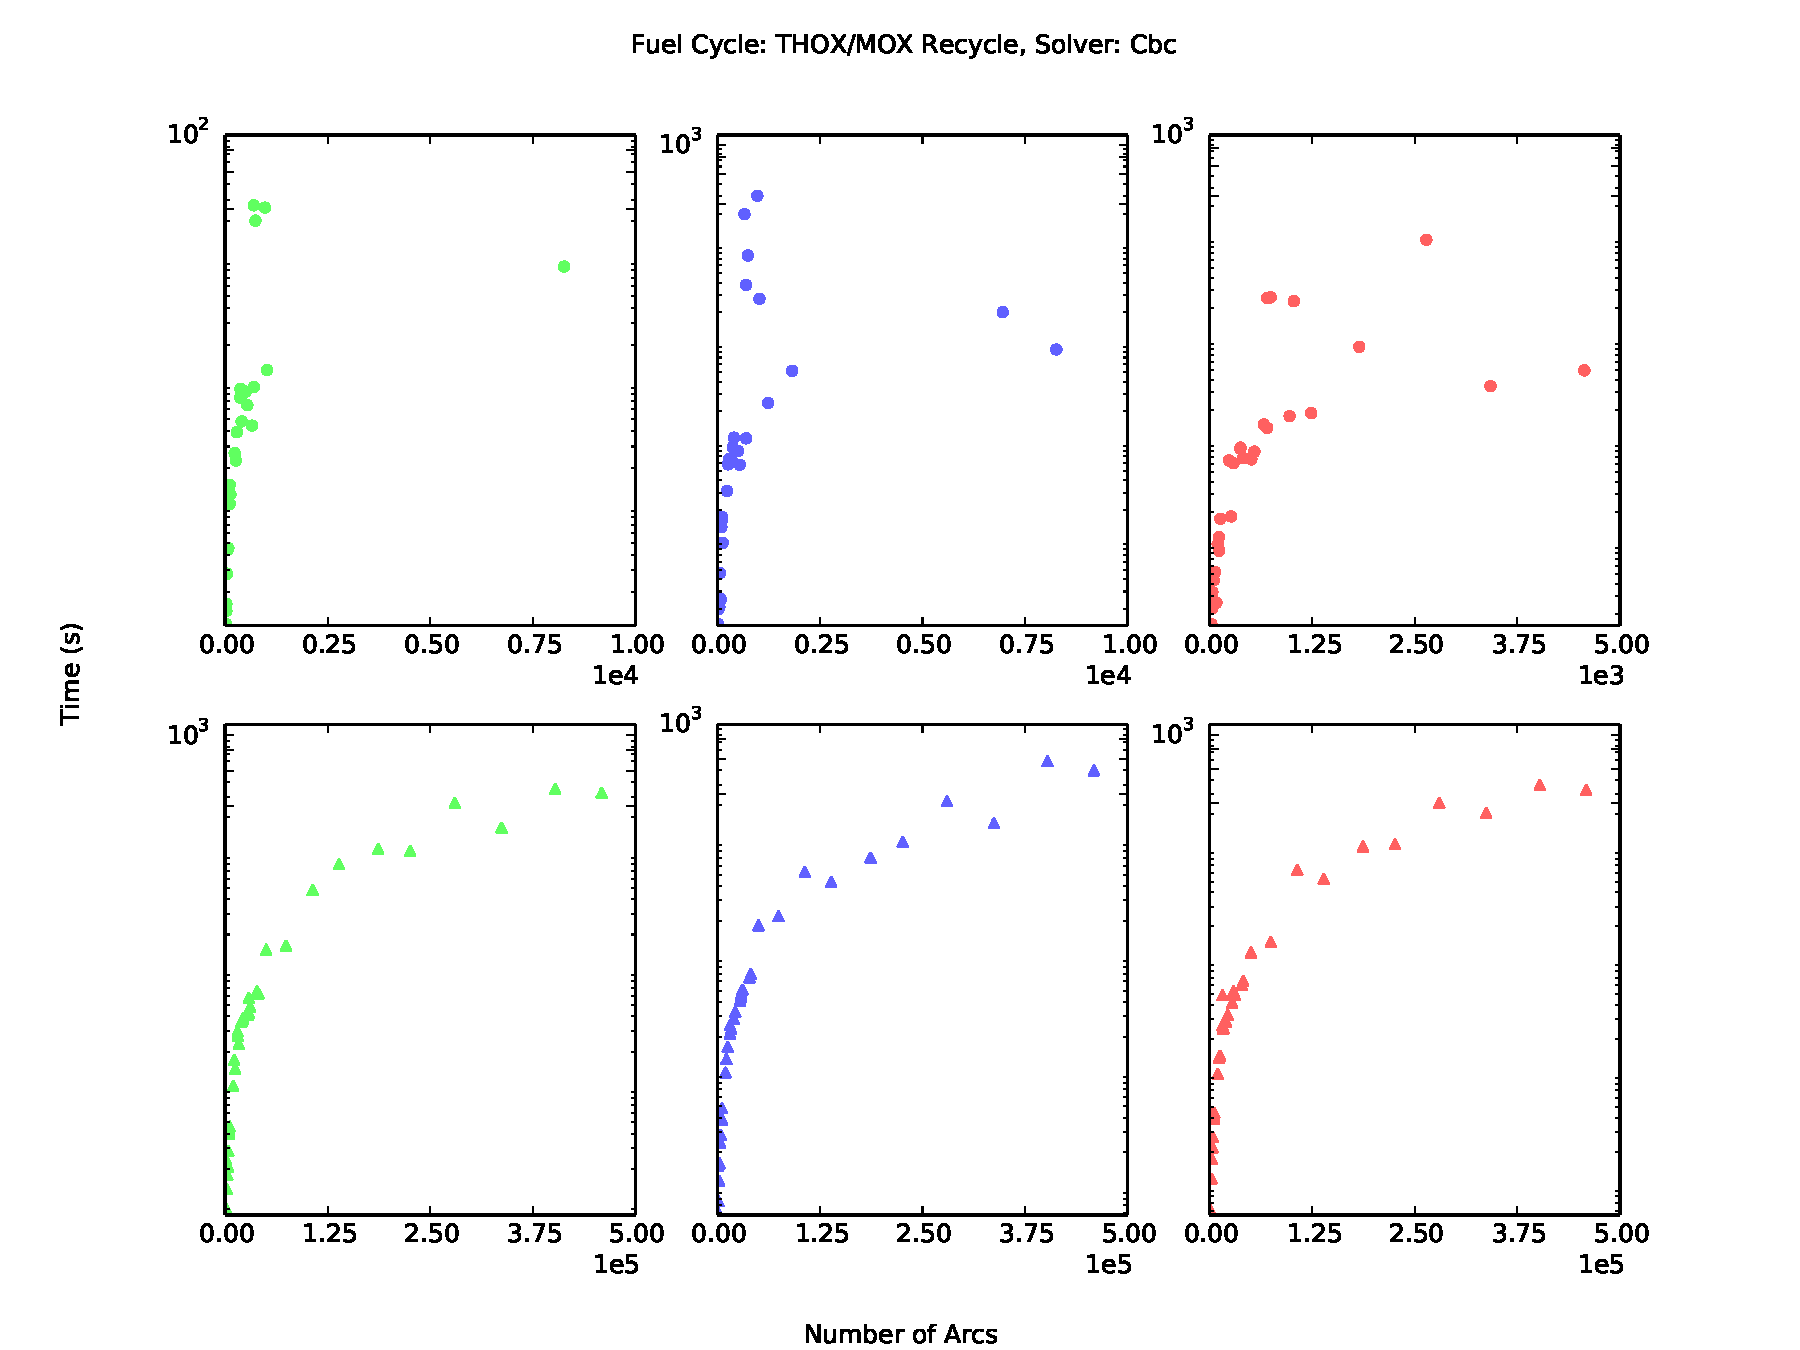
\includegraphics[width=.7\textwidth]{base_front_n_arcs_time_fc2_solvercbc.pdf}
    \caption[]{
      \label{fig:base_front_n_arcs_time_fc2_solvercbc}
      CBC Solver results for the ThOX fuel cycle as the number of arcs
      increases.
      }
  \end{center}
\end{figure}

Immediately obvious, and slightly counter intuitive, is that the population of
converged instances is larger for assembly-based exchanges rather than
batch-based exchanges, even though the number of variables in the problem is
much lower for batch-based exchanges. 

\TODO{More Explanation..}

%% \subsubsection{Instance Parameter Variation}
%% % Include large and small r_l_c

%% \paragraph{Location-to-Commodity Importance Ratio}

%% \paragraph{Thermal and Fast-Reactor Populations}

%% \paragraph{Inventory vs. Processing Constraints}

\subsubsection{Solution Comparison}\label{sec:res:scale:front:soln}

Solutions between any two solvers can be compared either in the formulation
layer or in the exchange layer. Comparison in the formulation layer is achieved
by comparing objective function values (Equation \ref{eqn:obj_flow}), whereas
comparison in the exchange layer is achieved by comparing a measure the flows
and preferences for a given solution (Equation \ref{eqn:sim_flow}). The
objective function includes the costs and flows on false arcs which can largely
inflate the objective function value. While the false arcs are necessary for
guaranteeing a feasible solution, their resulting flows are not taken into
account when the DRE back-translates from the formulation to the exchange
layer. Accordingly, a measure of the preference and flow, as shown in Equation
\ref{eqn:sim_flow}, is used to compare results between solvers. 


Comparisons are made between the Greedy solver and the CBC solver when the CBC
solver, provided the CBC solver converged. Because solutions increase in
magnitude with increasing problem size, a relative comparison is made, as shown
in Equation \ref{eqn:sim_flow_compare}. The resulting features are similar
across fuel cycles. Accordingly, an exmaple for the MOX fuel cycle is shown in
Figure \ref{fig:compare_cbc_greedy_pref_flow_front_n_rxtr__fc1_}.

\begin{equation}\label{eqn:sim_flow_compare}
\frac{z_{\text{sim}, \text{CBC}} - z_{\text{sim}, \text{Greedy}}}
     {z_{\text{sim}, \text{CBC}}} 
\end{equation}

\begin{figure}[h!]
  \begin{center}
    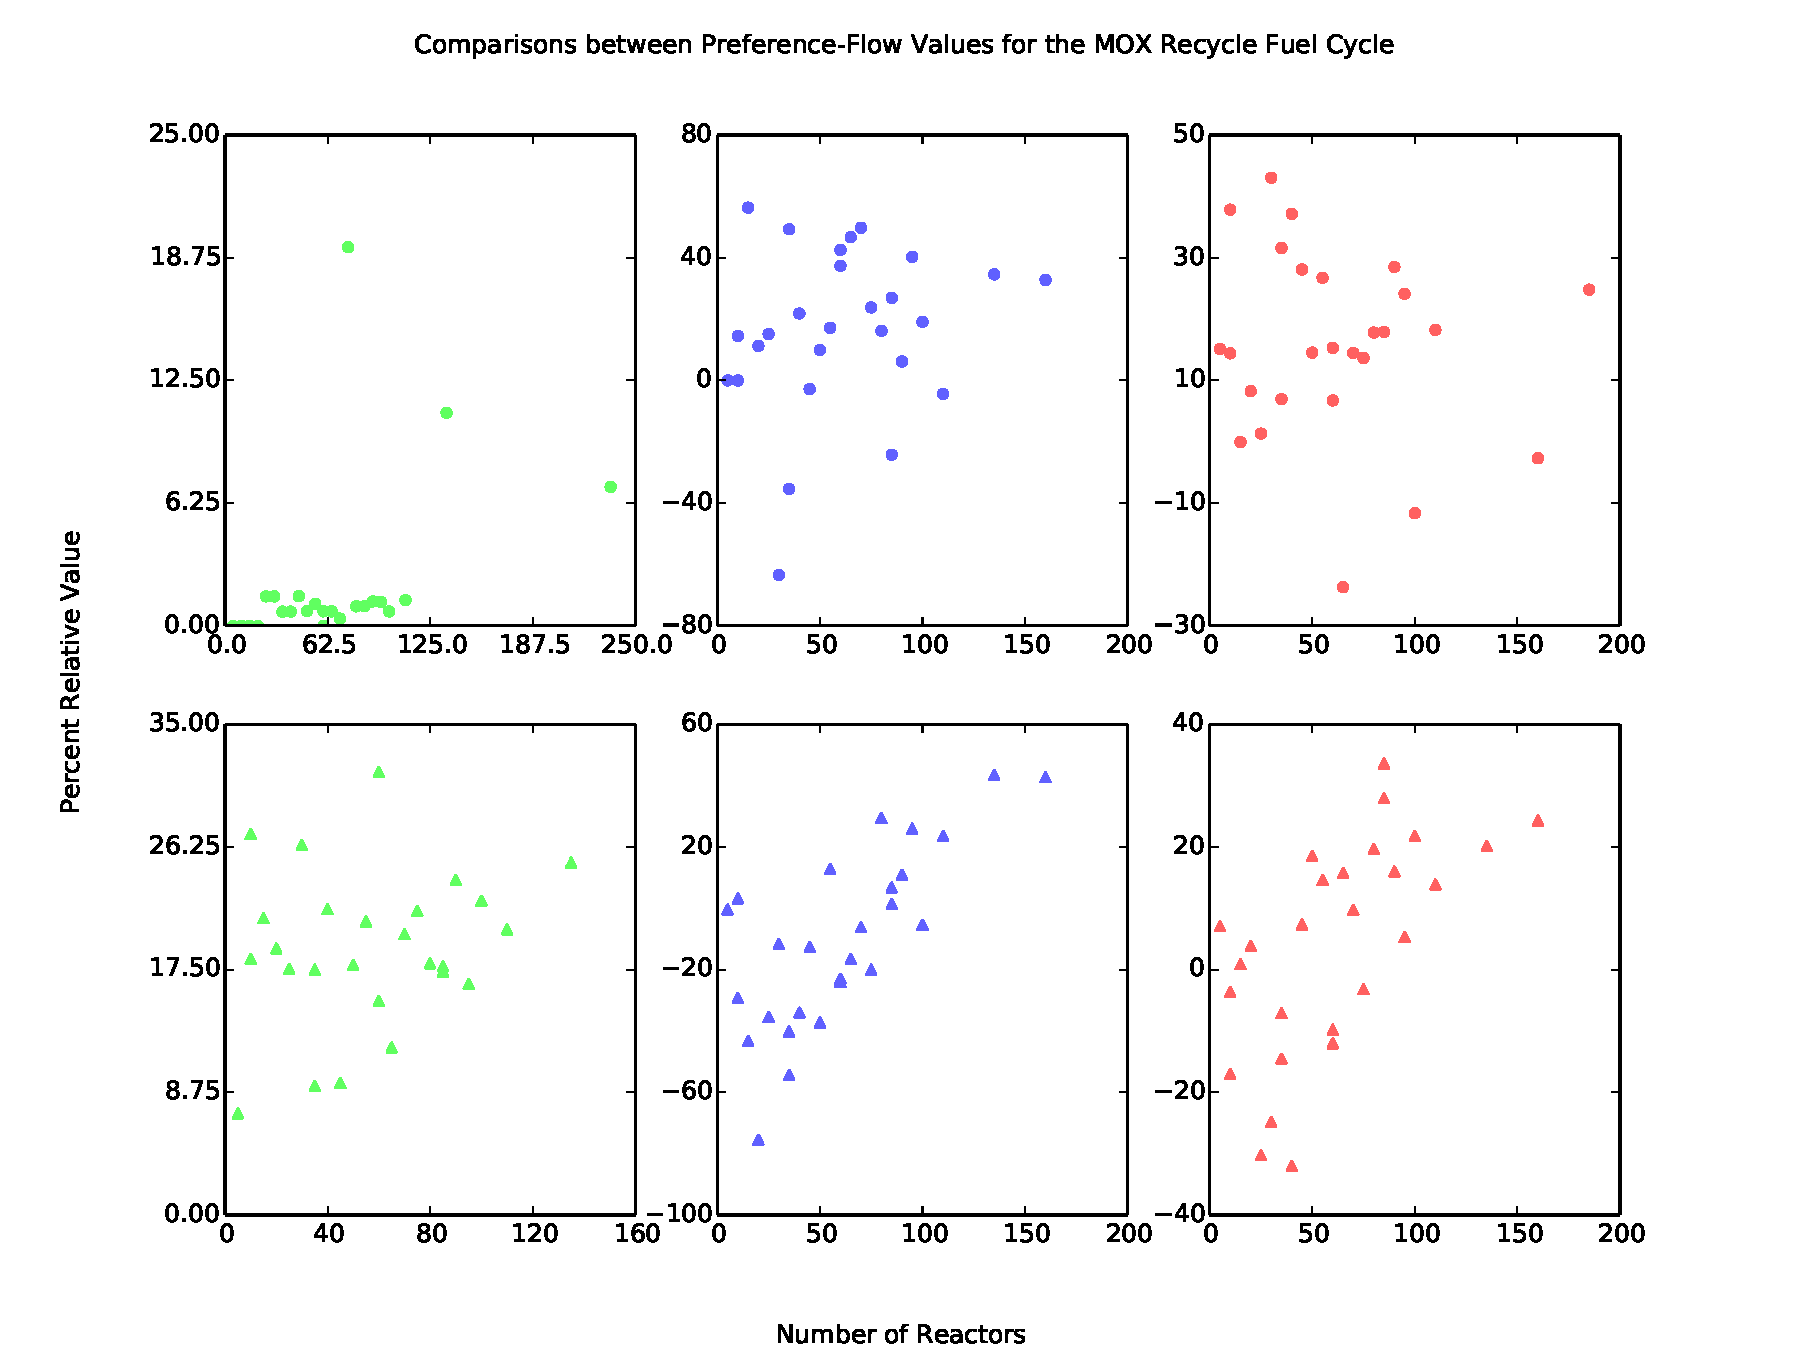
\includegraphics[width=.7\textwidth]{compare_cbc_greedy_pref_flow_front_n_rxtr__fc1_.pdf}
    \caption[]{
      \label{fig:compare_cbc_greedy_pref_flow_front_n_rxtr__fc1_}
      Comparisons between relative simulation metrics between the CBC solver and
      the Greedy solver for MOX fuel cycles. Only converged CBC
      solutions are compared.  }
  \end{center}
\end{figure}

Comparing the results in which there are no location-based preferences (the
green data points), there is a clear correlation between the number of variables
and the relative benefit of using CBC. Thus, the Greedy heuristic performs
better when the number of possible assignments is small. As more variety is
included in objective coefficient values via location assignment, the spread of
possible values increases -- the objective function projection on the feasible
space gains more features. 

Comparing the cases in which there is a coarse location preference (the blue
data points) and a fine location preference (the red data points), two features
of interest arise. First, some values are negative, implying that the Greedy
solver provides a better preference-space solution than the CBC
solver. Importantly, this is true only in preference space; the CBC always
performs better in cost space, by definition. The Greedy solver is allowed to
provide better answers in preference space for two reasons: the problem is
highly constrained, and false arcs have an arbitrarily high unit cost. CBC will
converged when the gap between the upper and lower bound on the optimal solution
reaches a small enough gap, $r^*$, as shown in Equation
\ref{eqn:ratio_gap}. Further, when a problem is highly constrained, many false
arcs will be activated, contributing a large amount to the objective
function. If the choice between two possible flows is sufficiently small, i.e.,
small relative to $z^*$, then either solution may be returned upon convergence
depending on the branch-and-bound search path. Thus, good solutions in
preference-space are somewhat lost in the ``noise'' of cost-space.

\begin{equation}\label{eqn:ratio_gap}
\frac{z^*_U - z^*_L}
     {z^*_U} \leq r^*
\end{equation}

This effect is clearly reduced when the objective choice in cost-space increase,
as shown in case of fine location preference. In short, the objective function
has a more pronounced shape in cost-space, reducing the heuristic quality and
increasing the quality of the CBC solution. Interestingly, as can be seen in the
lower part of Figure \ref{fig:compare_cbc_greedy_pref_flow_front_n_rxtr__fc1_},
as the number of variables increases (and the quantity associated with each
variable decreases), CBC performance decreases. Effectively, more false-arc
quantity can be packed into the solution because there is finer-grained choice
for assembly requests than for batch requests.

As previously described, the Greedy solver can provide quite good
preference-space results relative to the CBC solver when an exchange is highly
constrained \textit{and} when the cost coefficient assigned to false arcs is
relatively large. This effect can be observed by adjusting the false-arc cost
coefficient, e.g., as shown in Equation \ref{eqn:small_false_cost}. Two
exchanges for which the Greedy solver performed better in preference-space were
chosen to demonstrate the effect. The results are shown in Table
\ref{tbl:false_arcs}. Note that it every case, $z$ is smaller for the Greedy
solver than CBC; however, $z_\text{sim}$ for the Greedy solver is larger than
the same value with a large CBC false-arc cost and smaller than values related
to small CBC false-arc costs.

\begin{equation}\label{eqn:small_false_cost}
c_\text{false} = \frac{1}{p_\text{max}} + 1
\end{equation}

\begin{table}[h!]
\centering
\caption{Results from Reducing False-Arc Cost Coefficients.}
\label{tbl:false_arcs}
\begin{tabular}{|c|c|c|c|c|c|c|}
\hline
\multirow{2}{*}{\textbf{Simulation ID}} 
& \multicolumn{2}{c|}{\textbf{Greedy}} 
& \multicolumn{2}{c|}{\textbf{CBC, Large Cost}} 
& \multicolumn{2}{c|}{\textbf{CBC, Small Cost}} \\ \cline{2-7} 
& $z$ (large/small)        & $z_{\text{sim}}$        
& $z$             & $z_{\text{sim}}$            
& $z$             & $z_{\text{sim}}$            \\ \hline
54a5a92ce1ad43e9a713abf114b58a06
& 5.2e8/1.9e6 & 1.41e5
& 5.0e8 & 1.38e5
& 1.8e6 & 1.98e5 \\ \hline
938d808a4bd84346b54f38fcb4992386
& 3.97e8/1.40e6 & 1.08e5
& 3.81e8 & 8.8e4
& 1.38e6 & 1.12e5 \\ \hline
\end{tabular}
\end{table}

\subsubsection{Convergence Criteria}

The CBC solver, and MILP solvers in general, is highly tuneable. Perhaps the
most critical tuneable criteria affecting the balance between solution quality
and solution time is the convergence criteria. It is not clear to what degree
solution quality will matter for users of Cyclus. Accordingly, a short
exploratory experiment was conducted to examine to what degree convergence
criteria affects solution time.

CBC uses either an absolute or relative upper and lower-bound gap tolerance as
possible convergence criteria. All results discussed use the relative gap,
termed \textit{ratio gap} in CBC parlance, as shown in Equation
\ref{eqn:ratio_gap}. For each of the 18 combinations of fundamental parameters,
10 instances of exchanges were executed, spanning a reactor population range of
10 to 500. Figure \ref{fig:hist_front_rxtr_0} displays the results for runs with
reactors trading full batches for ratio gap values of 0.1, 1, and 10\%. Figure
\ref{fig:hist_front_rxtr_0} displays the results for runs with reactors trading
individual assemblies for ratio gap values of 1 and 10\%.

\begin{figure}[h!]
  \begin{center}
    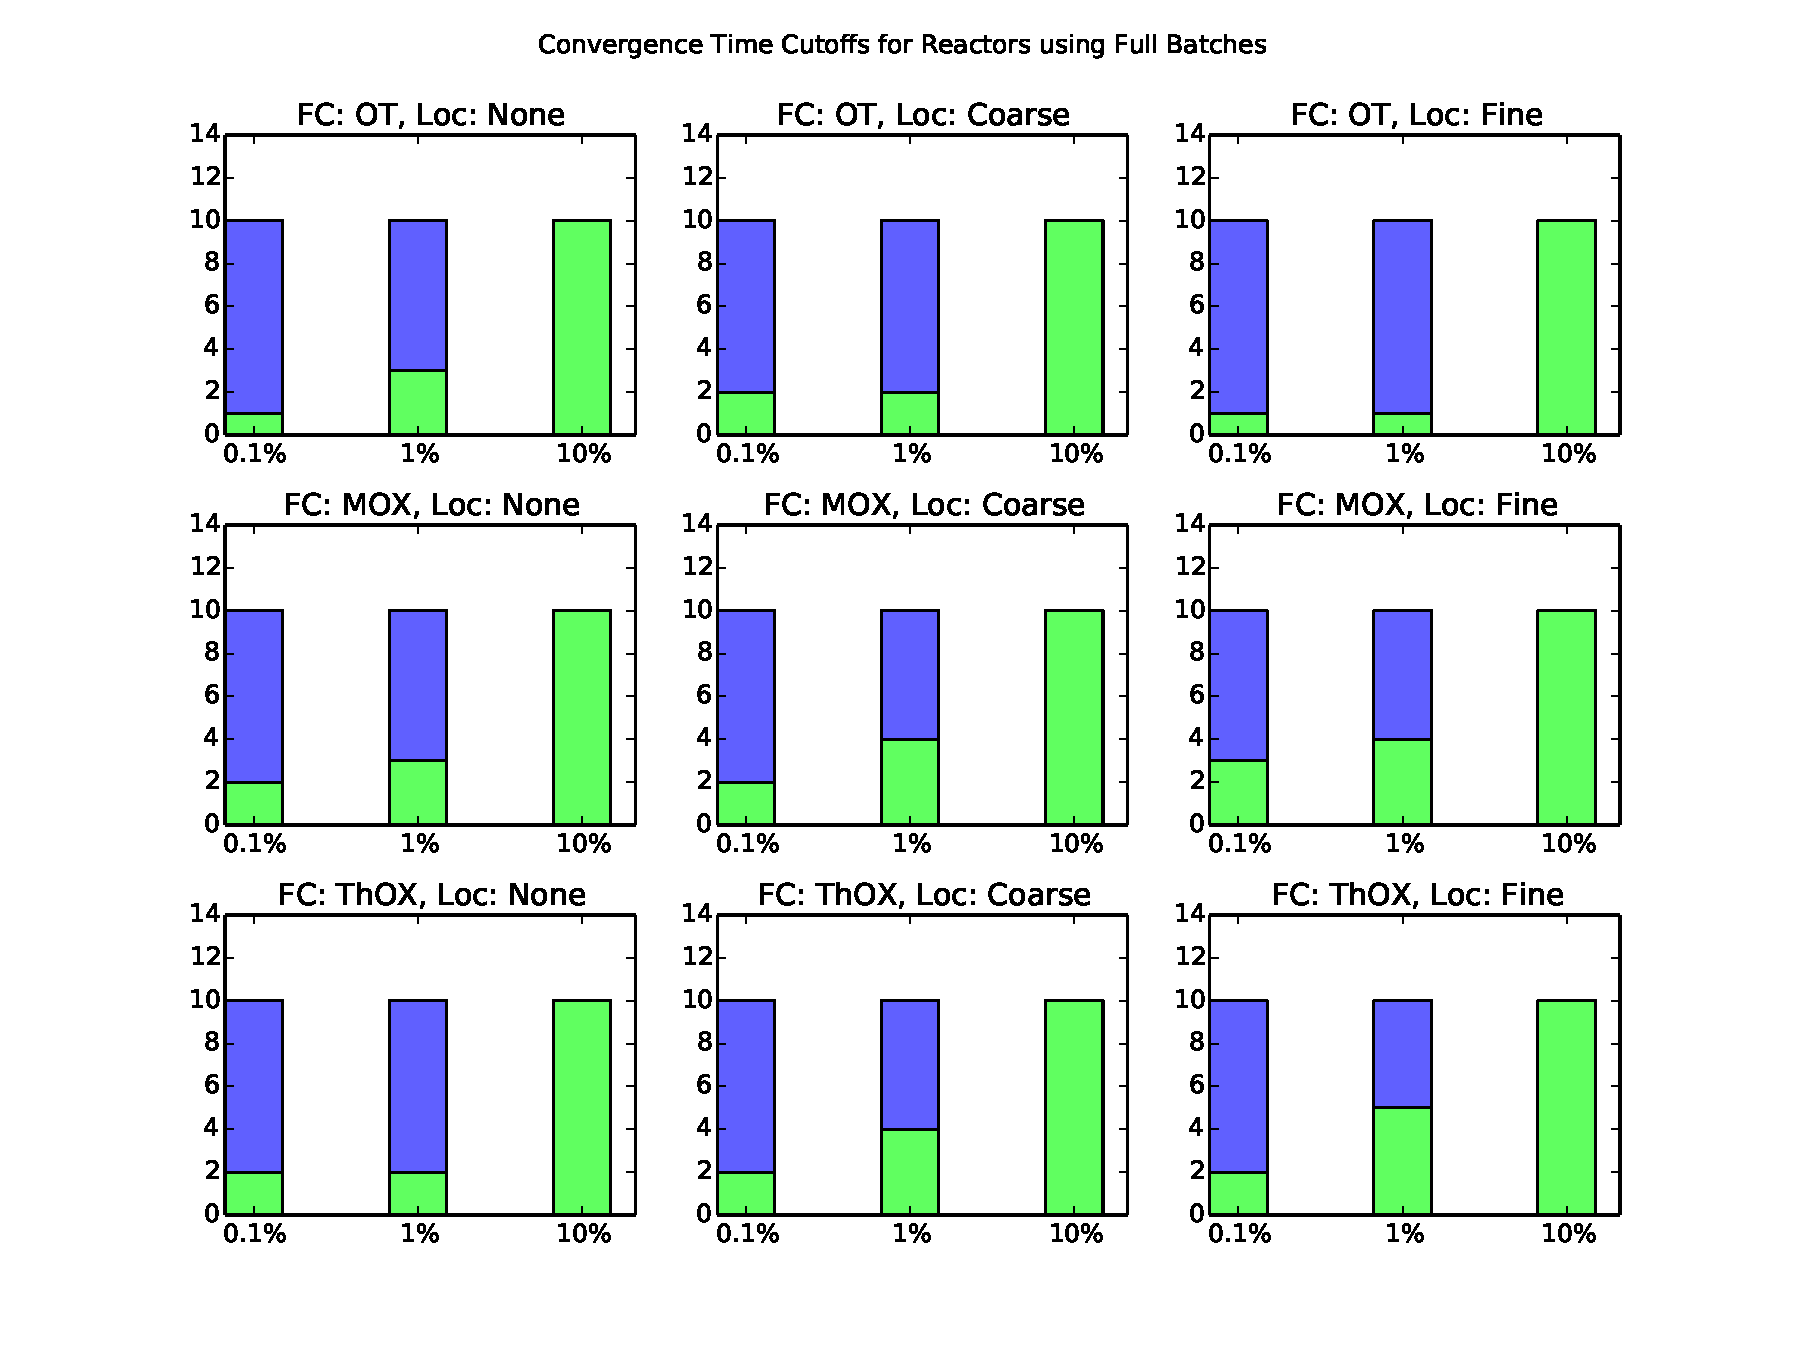
\includegraphics[width=.95\textwidth]{hist_front_rxtr_0.pdf}
    \caption[]{
      \label{fig:hist_front_rxtr_0}
      Effects of increasing convergence criteria on Front-End exchanges with
      reactors exchanging batches. Each bar is divided into how many instances
      converged (green) and did not converge (blue). }
  \end{center}
\end{figure}

\begin{figure}[h!]
  \begin{center}
    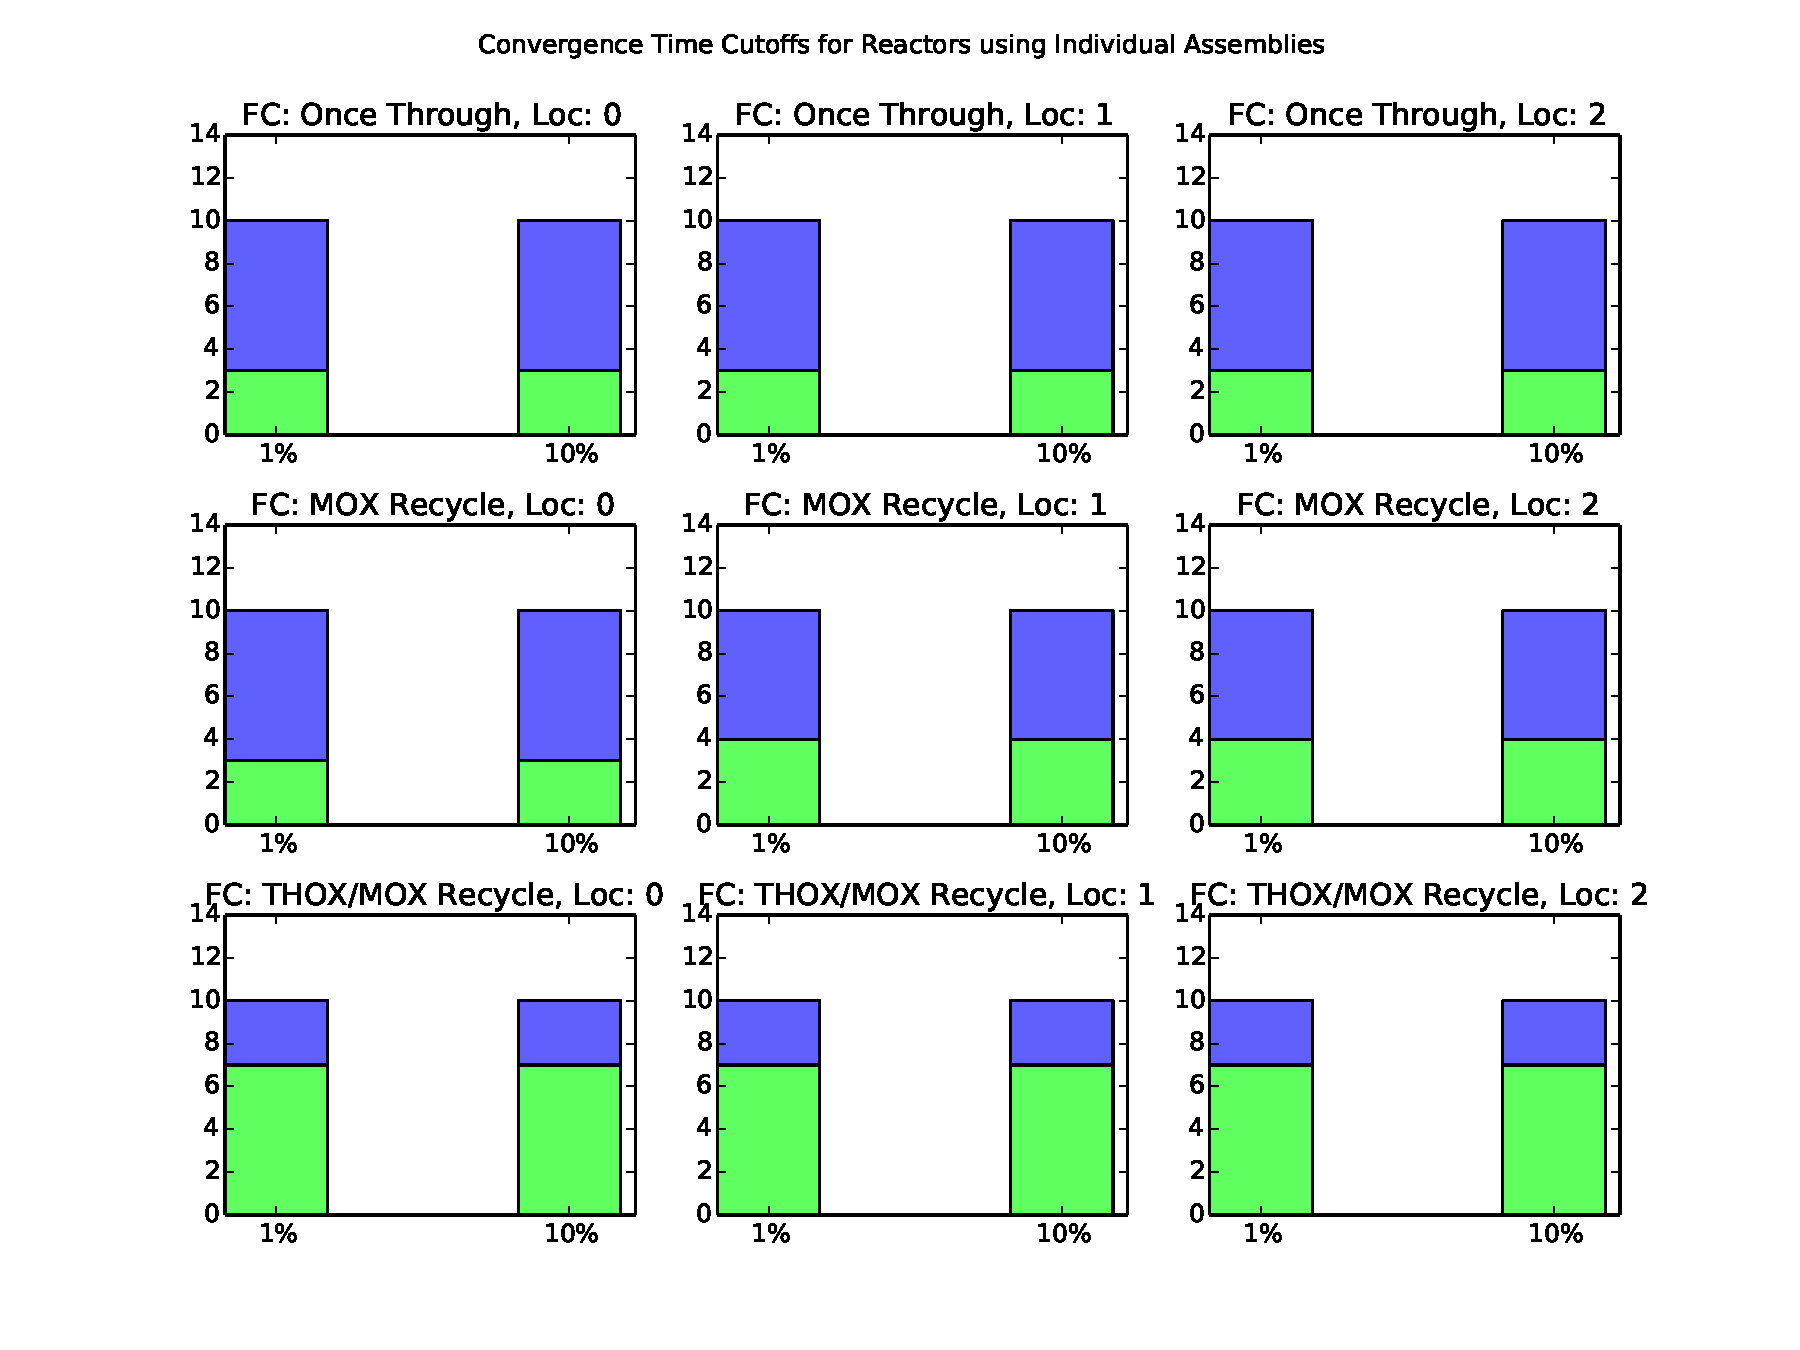
\includegraphics[width=.95\textwidth]{hist_front_rxtr_1.pdf}
    \caption[]{
      \label{fig:hist_front_rxtr_1}
      Effects of increasing convergence criteria on Front-End exchanges with
      reactors exchanging assemblies. Each bar is divided into how many instances
      converged (green) and did not converge (blue).}
  \end{center}
\end{figure}

Increasing the convergence criteria for smaller problems has a greater effect
than increasing the convergence criteria for larger probems. It is somewhat
surprising that the increase from a 1\% relative bound gap to a 10\% gap allows
full convergence in the smaller case and has no effect in the larger
case. Considering the discussion in \S \ref{sec:res:scale:front:soln}, it is
likely that the large convergence effect is due increasing the ``noise'' effect
of actual arcs. However, users will likely find some speed ups in solution times
by relaxing convergence criteria, and those speed ups will likely be more
profound in smaller-sized problems than larger problems.

\subsection{Back-End Exchanges}

Many of the results of the back-end exchanges mirror those of the front-end
exchanges. Specifically, 

\subsubsection{Reference Case}



\begin{figure}[h!]
  \begin{center}
    \includegraphics[width=.7\textwidth]{base_back_n_rxtr_n_arcs_fc1_solvergreedy.pdf}
    \caption[]{
      \label{fig:base_back_n_rxtr_n_arcs_fc1_solvergreedy}
      Arc population scaling with the number of reactors with coresponding linear fits.}
  \end{center}
\end{figure}

\begin{figure}[h!]
  \begin{center}
    \includegraphics[width=.7\textwidth]{base_back_n_rxtr_n_constrs_fc1_solvergreedy.pdf}
    \caption[]{
      \label{fig:base_back_n_rxtr_n_constrs_fc1_solvergreedy}
      Constraint population scaling with the number of reactors with
      corresponding quadratic fits.}
  \end{center}
\end{figure}


%% \subsubsection{Instance Parameter Variation}
%% % Include large and small r_l_c

%% \paragraph{Location-to-Commodity Importance Ratio}

%% \paragraph{Thermal and Fast-Reactor Populations}

\subsubsection{Convergence Criteria}
